\documentclass{article}
\usepackage[utf8]{inputenc}

\usepackage{tabularx}
\usepackage{graphicx}
\usepackage{adjustbox}
\usepackage{hyperref}
\usepackage{etoolbox}
\usepackage{changepage}
\usepackage{float}
\usepackage{amsmath}

\usepackage[margin=0.75in]{geometry}

\usepackage[disable]{todonotes}
%use this line instaed to hide todo's
%\usepackage[disable]{todonotes}

\usepackage{cleveref}

\title{Halbleiterphysik Fragenkatalog}
\author{Constantin Schieber\\Benedikt Tutzer}
\date{August 2020}

%\patchcmd{\subsubsection}{\normalsize}{\normalsize}{\typeout{same line subsec f}}{\typeout{same line subsec failed}}%
%\patchcmd{\subsubsection}{\bfseries}{}{\typeout{same line subsec f}}{\typeout{same line subsec failed}}%

\newtoggle{aftersection}
\preto{\section}{\filbreak\global\toggletrue{aftersection}}
\preto{\subsection}{\iftoggle{aftersection}{\global\togglefalse{aftersection}}{\filbreak}}
\newcommand{\clearpageafterfirst}{%
  \gdef\clearpageafterfirst{\clearpage}%
}


\begin{document}


\maketitle
\vfill
Diese Ausarbeitung ist zur Vorbereitung auf die m\"undliche Pr\"ufung im August 2020 entstanden. Sie kann gern auf overleaf aktuell gehalten werden.\\

\begin{center}\href{Overleaf public link}{https://www.overleaf.com/4852512811wdbqyxrbkgyb}\end{center}

\newpage
\tableofcontents
\newpage

%--------------------------------------------------------------------------------
%--------------------------------------------------------------------------------
%--------------------------------------------------------------------------------
\section*{Overview}
\addcontentsline{toc}{section}{Overview}    %Makes the above section appear in the table of contents


\begin{center}
\begin{table}[H]
%\begin{adjustwidth}{-3cm}{-3cm}
\begin{adjustbox}{width=\textwidth}
\centering
\begin{tabular}{lcccccccc}
Frage                & 02.16 & 01.28 & 02.19 & 03.04 & 03.05 & 03.21 & 01.16 & Katalog\\
                     & 2010  & 2014  & 2019  & 2019  & 2019  & 2019  & 2020 & \\
                     \hline
\ref{k1:photoEf} Photo-Effekt &&&&&&&& X \\
\ref{k1:comptonEf} Compton-Effekt &&&&&&&& X \\
\ref{k1:dispersionsrelation} Dispersionsrelation für Halbleiter && X &&& X & X & X & \\
\ref{k1:schrGl} Schrödinger Gleichung&&&& X &  & X & X & X \\
\ref{k1:ekdiag} e(k) Diagramm &&&&&&&& X \\
\ref{k1:pottopf} Unendlich tiefer Potentialtopf & X &&&&&&& X \\
\ref{k1:tunnEf} Tunneleffekt&&&& X &&&X & \\
\ref{k2:metalle} Unterschied Halbleiter vs Metalle &&&&&&&& X\\
\ref{k2:festkorper} Grund für Festkörperbildung & X &&&&&&& X\\
\ref{k2:leitungsBand} Leitungsband, Valenzband, Ef aufzeichnen && X & X &&&&& \\
\ref{k2:kroningpenny} Kroning Penny Modell &&&&&&&& X \\
\ref{k2:entstehungHalbleiter} Enstehung der Halbleiter &&&&&&&& X \\
\ref{k2:phononen} Phononen &&&&&&&& X \\
\ref{k3:diffusion} Berechnung Diffusionsspannung & X &&&&&&& X \\
\ref{k3:alleGleichungen} Alle Gleichungen & X &&&&&&& \\
\ref{k3:dotieren} Dotieren &&&&&&&& X \\
\ref{k3:ladungstraegerkonz} Verlauf der Ladungstr\"agerkonzentration &&&&&&&& X \\
\ref{k3:drude} Drude Modell &&&&&&&& X \\
\ref{k3:halleffekt} Hall-Effekt &&&&&&&& X \\
\ref{k3:hallspannung} Hall-Spannung &&&&&&&& X \\
\ref{k3:diffusionsstrom} Diffusionsstrom &&&&&&&& X \\
\ref{k3:stromgleichungen} Stromgleichungen, J\_n, J\_p &&&&&&&& X \\
\ref{k3:shockleyhaynes} Shockley-Haynes Experiment &&&&&&&& X \\
\ref{k3:kontinuitaet} Kontinuit\"atsgleichungen &&&&&&&& X \\
\ref{k4:laser} Wie funktionieren Laser & X &&&&&&& X\\
\ref{k4:inUndIndirekt} Direkter und Indirekter Halbleiter&&& X &&&&& X \\
\ref{k4:zustandsDichte} Zustandsdichte und Besetzungswahrscheinlichkeit && X &&&&& X \\
\ref{k5:pn} PN-\"Ubergang && X & X & X &X&X&& X \\
\ref{k5:diode} Diodenkennlinie &&&&&&&& X \\
\ref{k5:pnBand} Banddiagramm f\"ur PN ohne Spannung  && X &&&&&& \\
\ref{k5:schottky} Schottky-Kontakt-Diode &&&&&&&& X \\
\ref{k5:tunnelDiode} Tunneldiode&&& X && X & X & X & X \\
\ref{k5:backward} Backward-Diode &&&&&&&& X \\
\ref{k5:heterostrukturen} Heterostrukturen &&&&&&&& X \\
\ref{k6:bipolar} Funktion von Bipolartransistoren & X &&&&&&& X \\
\ref{k6:mosInversion} MOS-Struktur & X && X &&&&& \\
\ref{k6:diffusionsdreieck} Diffusions-Dreieck beim Transistor &&&&&&&& X \\
\ref{k6:fet} Feldeffekt-Transistor &&&&&&&& X \\
\ref{k6:mosfet} MOS-FET &&&&&&&& X \\
\ref{k6:mesfet} MES-FET &&&&&&&& X \\
\ref{k6:early} Early-Effekt &&&&&&&& X \\
\ref{k6:jfet} JFET &&&&&&&& X \\

\hline

\hline

\end{tabular}
\end{adjustbox}
%\end{adjustwidth}
\caption{Mündliche Prüfungsfragen aus diversen Aufzeichnungen der FET.}
\end{table}
\end{center}

%--------------------------------------------------------------------------------
%--------------------------------------------------------------------------------
%--------------------------------------------------------------------------------
\section{Physikalische Grundlagen - Kapitel 1}
\subsection{Photo-Effekt \todo{0x}}\label{k1:photoEf}
Wenn Licht auf reine Metalle trifft und dabei die Frequenz des Lichts eine gewisse Schwelle überschreitet werden Elektronen aus dem Metall gelöst.

\begin{figure}[H]
    \centering
    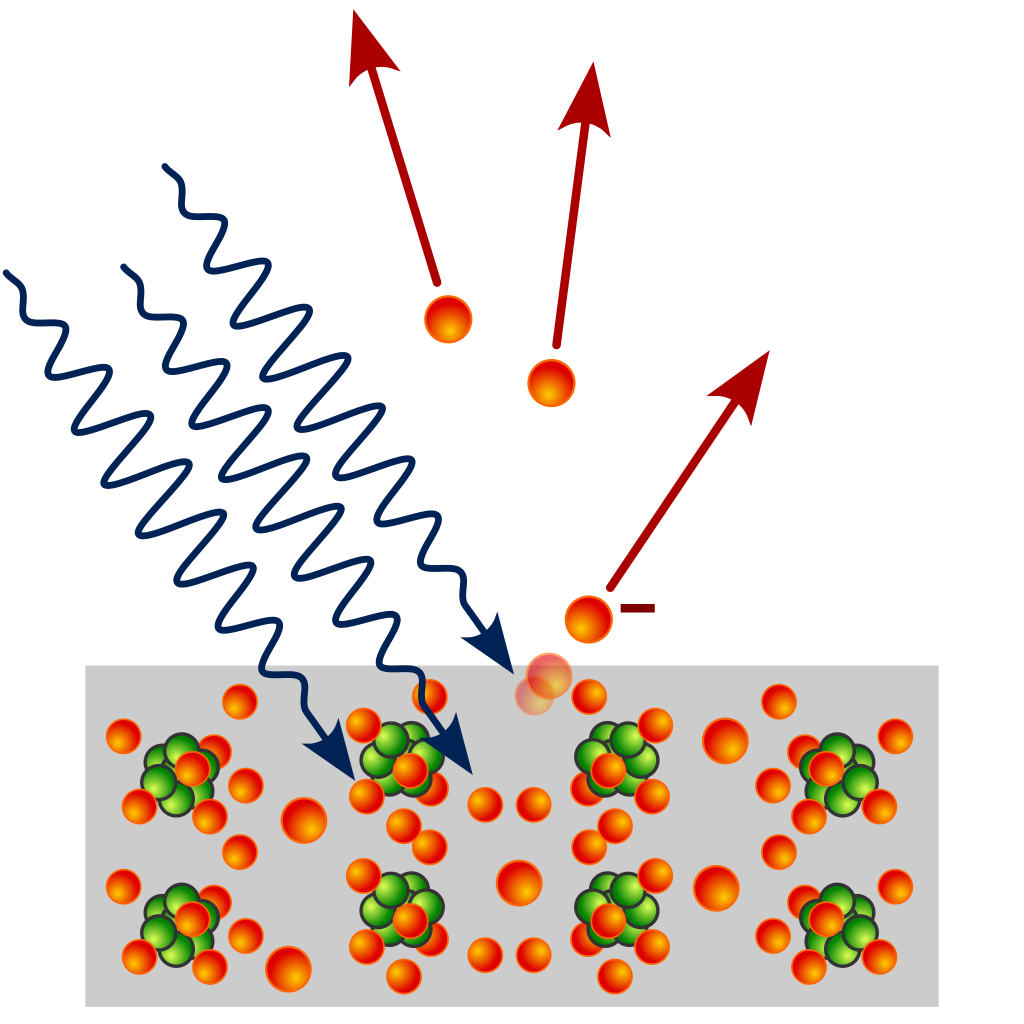
\includegraphics[width=0.33\textwidth]{fig/photoeffect}
    \caption{Photoeffekt}
    \label{fig:photoeffect}
\end{figure}

\subsubsection{Austrittsarbeit}
Die Energie von Licht hängt mit dessen Frequenz zusammen: $\hbar \cdot f$
Die Zahl der emittierten Elektronen ist proportional zur Energie des Lichts.

Das Elektron aus dem Metall muss zum Austreten die \textit{Austrittsarbeit}: $W = h \cdot f_g$ verrichten können.
Hat ein Photon also nicht mindestens die Frequenz $f_g$, oder besser noch $f > f_g$, dann kann auch kein Elektron freigesetzt werden.

Die Austrittsarbeit kann auch experimentell (Lenard, 1992) beobachtet werden: $e|U| = h| f - f_g|$
\begin{figure}[H]
    \centering
    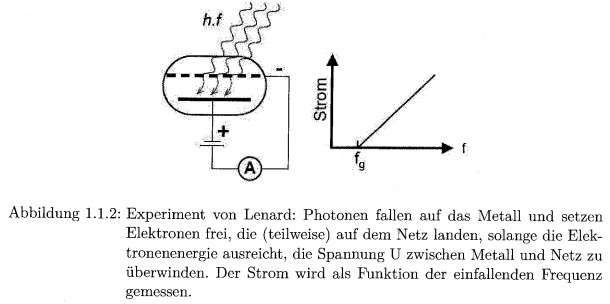
\includegraphics[width=0.5\textwidth]{fig/photoExperiment}
    \caption{Photoeffekt}
    \label{fig:photoeffectExperiment}
\end{figure}

\subsection{Compton-Effekt \todo{0x}}\label{k1:comptonEf}
UV-Licht trifft auf Metall. Im Streulicht (der Reflexion), ist dann nicht nur die Primärfrequenz sondern auch noch längerwellige Frequenz nachweisbar.   
Compton Effekt (eben das Auftreten dieser längerwellige Frequenz) ist nicht allein durch das Wellenbild des Photons erklärbar.
Über das Teilchenbild ist das Phänomen allerdings vollständig erklärbar indem man den elastischen Stoß zwischen Photon und Elektron betrachtet.

\begin{figure}[H]
    \centering
    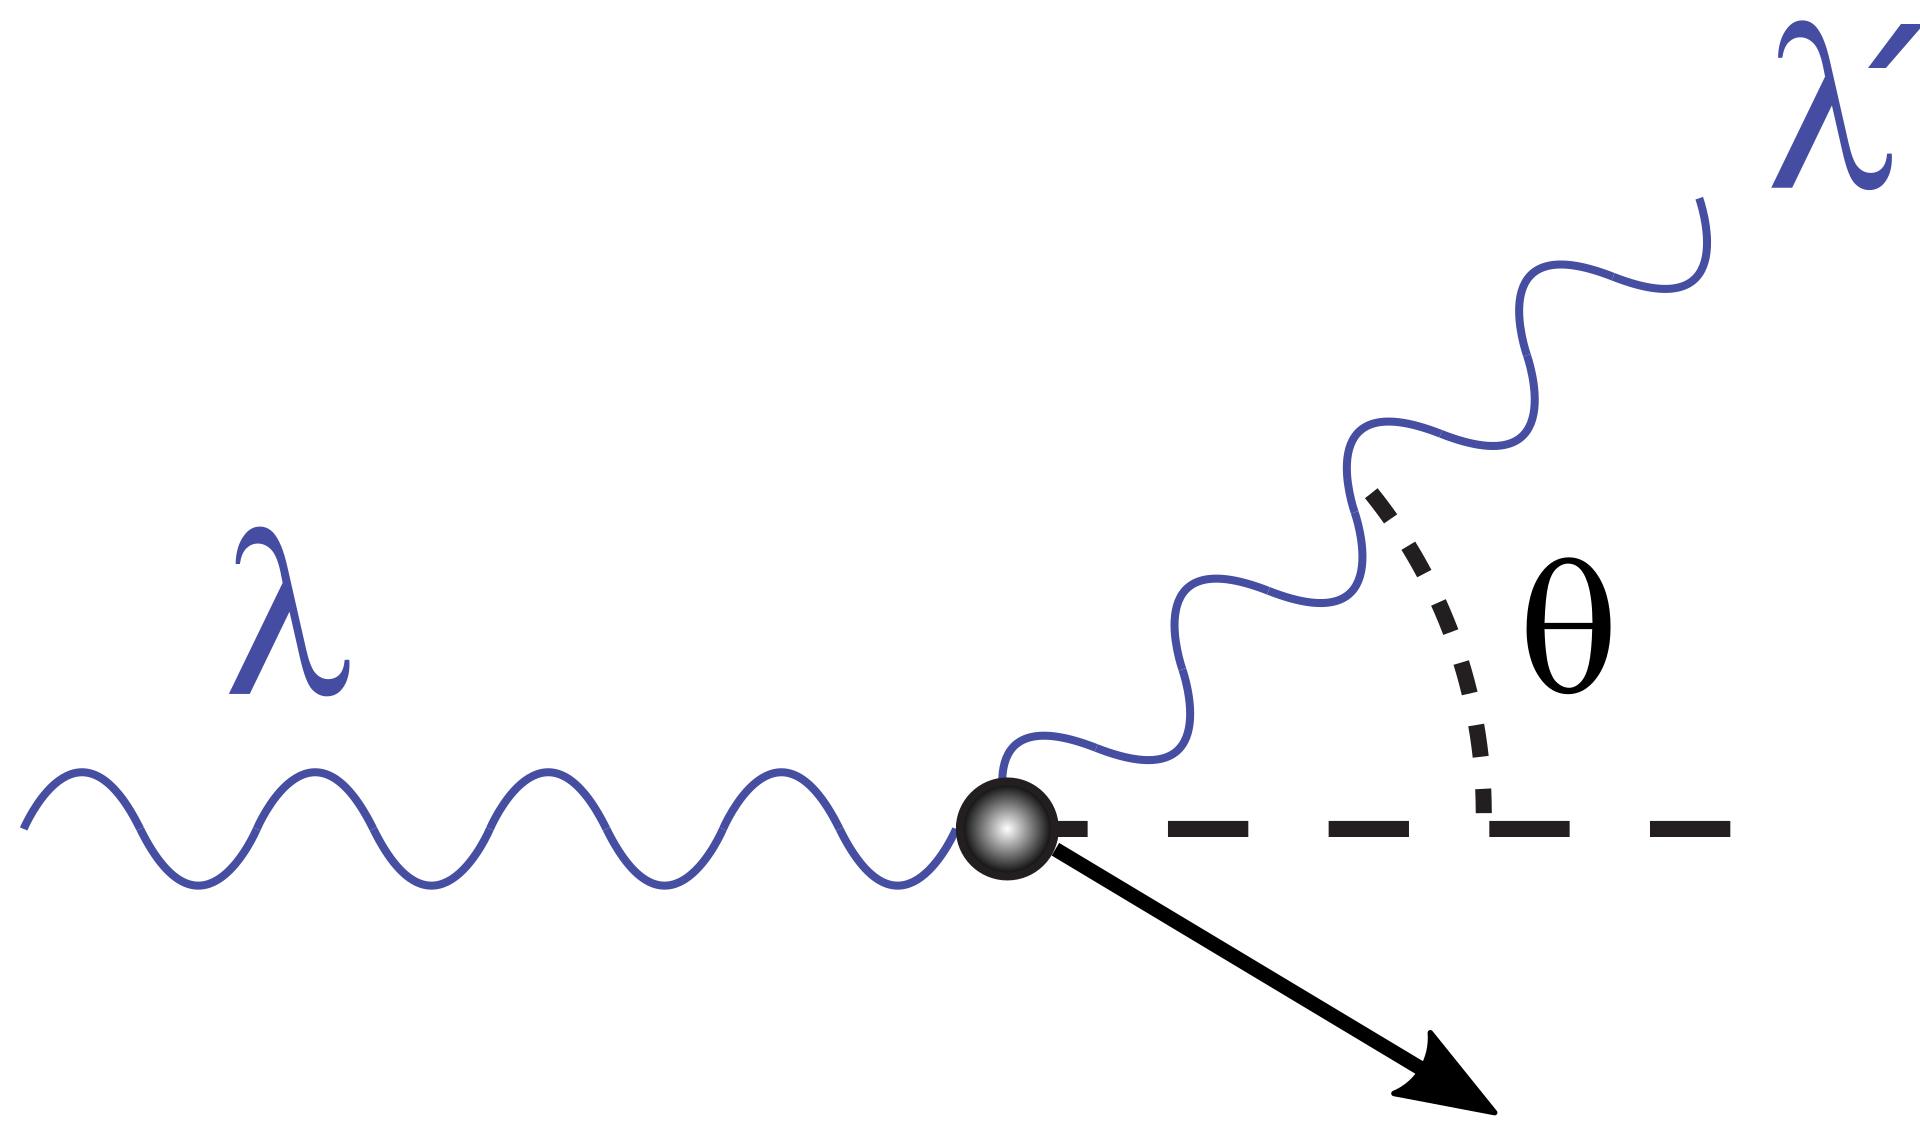
\includegraphics[width=0.5\textwidth]{fig/compton}
    \caption{Compton-Effekt}
    \label{fig:comptonEffect}
\end{figure}

\subsubsection{Durch welche zwei Gleichungen lässt sich der Compton-Effekt erklären?}
Durch den Energie und Impulserhaltungssatz. 

\begin{enumerate}
    \item $E_e$ ... kinetische Energie
    \item $\vec{p}_e$ ... Impuls des Compton-Elektrons (welches heraus geschlagen wird)
    \item $\vec{k}$ ... Wellenvektor zeigt die Ausbreitungsrichtung des Photons
\end{enumerate}
\begin{equation}
    \hbar \omega_0 = \hbar \omega_{sc} + E_e
\end{equation}

\begin{equation}
    \hbar \vec{k}_0 = \hbar \vec{k}_{sc} + \vec{p}_e
\end{equation}

\subsubsection{Was beweist der Compton-Effekt?}
Der Compton-Effekt ist ein direkter Beweis, dass Photonen nicht nur die Energie $\hbar \omega$, sondern auch den Impuls $\hbar k$ haben.

\subsection{Dispersionsrelation \todo{4x}}\label{k1:dispersionsrelation}
\subsubsection{Bandstruktur}
\subsubsection{Bandlücke}
\subsubsection{direkt/ indirket}
\subsubsection{Effektive Masse (was ist schwerer, Elektron im Leitungsband oder Loch im Valenzband?)}
\subsubsection{Wo liegt k=0, E=0 für dirket/indirekt}
\subsubsection{wo ist Elektron nach anheben ins Leitungsband bei indirektem HL (energetisch günstig!)}
\subsubsection{Gedankenexperiment: wenn Elektron in Leitungsband, und Valenzband voll besetzt, was passiert, wenn man HL abkühlt?}

\subsubsection{Zusammenhang zwischen Energie E und der Kreiswellenzahl k}
\subsubsection{Lösung für freies Teilchen}
\subsubsection{Dispersion im Halbleiter}

\subsubsection{Skizze Valenzband, Leitungsband, Ferminiveau}
\subsubsection{Direkter indirekter Halbleiter}
\subsubsection{E(k) Diagramm einzeichen k = 0 , E = 0}

\subsubsection{Elektronen und Löcher}
Was bewegt sich wie, Loch zu Elektron, Elektron zu Loch

\subsubsection{Effektive Masse, Definitionen, Masssen}


\subsection{Schrödinger Gleichung \todo{3x}}\label{k1:schrGl}
\subsubsection{Herleitung für freies Teilchen}
Basiert auf der Annahme dass Welle - Teilchen - Dualismus exisiert. 

Dann gilt nämlich sowohl $E = \hbar \omega$ als auch $p = \hbar * k$

\subsubsection{Spezialfall der Schrödingergleichung für ein \textit{freies} Teilchen:}
\begin{equation}
    -\frac{\hbar^2}{2m} \times \frac{\partial^2}{\partial x^2} \Psi(x,t)  = i \hbar \times \frac{\partial}{\partial t} \Psi(x,t)
\end{equation}

\subsubsection{Allgemeine Form der Schrödingergleichung für ein Teilchen:}

\paragraph{Für den eindimensionalen Fall:}
\begin{equation}
    -\frac{\hbar^2}{2m} \times \frac{\partial^2}{\partial x^2} \Psi(x,t) + V(x,t) \times \Psi(x,t) = i \hbar \times \frac{\partial}{\partial t} \Psi(x,t)
\end{equation}

\paragraph{Für den dreidimensionalen Fall:}

Einfach alles durch Vektoren austauschen mit: 

\begin{equation}
    \frac{\partial^2}{\partial x^2} \longrightarrow \frac{\partial^2}{\partial x^2} + \frac{\partial^2}{\partial y^2} + \frac{\partial^2}{\partial z^2} \equiv \Delta
\end{equation}
und 
\begin{equation}
    E = \frac{\vec{p}^2}{2m} + V(\vec{x})
\end{equation}
was dann schließlich einfach

\begin{equation}
    -\frac{\hbar^2}{2m} \times \Delta \Psi(\vec{x},t) + V(\vec{x},t) \times \Psi(\vec{x},t) = i \hbar \times \frac{\partial}{\partial t} \Psi(\vec{x},t)
\end{equation}
ergibt. Man sieht, es ändert sich eigentlich nicht viel - einfach aus dem Ort \textit{x} und dem Impuls \textit{p} einen Vektor machen und logisch durchgehen wo diese ersetzt werden müssen. 

\begin{enumerate}
    \item Warum kann das Potential nicht von der Zeit abhängen
\end{enumerate}

\subsubsection{Dispersionsrelation für ein freies Teilchen}

\subsubsection{Aufstellen der Zeitabhängingen und Zeitunabhängigen Lösung}

\subsubsection{Einzelne Terme erklären}
\begin{enumerate}
    \item Was ist Phi
    \item Welche Abhängigkeiten (x, t) warum
    \item Was ist das Potenzial?
    \item Von was ist das Potenzial abhängig (x, t)
    \item Freies Teilchen in der Schrödingergleichung für V = 0
    \item Lösung der Schrödingergleichung für ein freies Teilchen im E(K) Diagramm
\end{enumerate}

\subsection{e(k) Diagramm \todo{0x}}\label{k1:ekdiag}
Das e(k) Diagramm beschreibt die Charakteristiken eines Halbleitermaterials. Abgebildet wird der Zusammenhang
zwischen Energie und Impuls von Quantenmechanischen Zuständen.
Ein Beispiel ist in \Cref{fig:ek} abgebildet.
\begin{figure}[H]
    \centering
    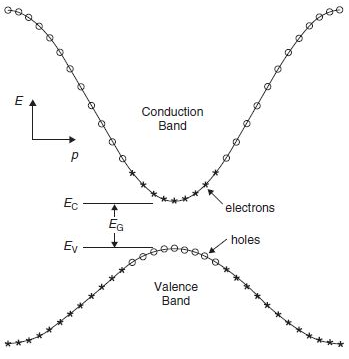
\includegraphics[width=0.3\textwidth]{fig/ek}
    \caption{Simples E-k Diagramm}
    \label{fig:ek}
\end{figure}
Man sieht:
\begin{itemize}
    \item Die Bandlücke $E_G$
    \item Die Effektive Masse anhand der Krümmung der beiden Kurven
    \item Die Zustandsdichte anhand der Steigung der beiden Kurven
\end{itemize}

\subsection{Unendlich tiefer Potentialtopf \todo{1x}}\label{k1:pottopf}
Der unendlich tiefe, rechteckige Potenzialtopf (\Cref{fig:pottopf}) ist ein sehr einfach zu lösender Spezialfall
der Schrödingergleichung.
\begin{figure}[H]
    \centering
    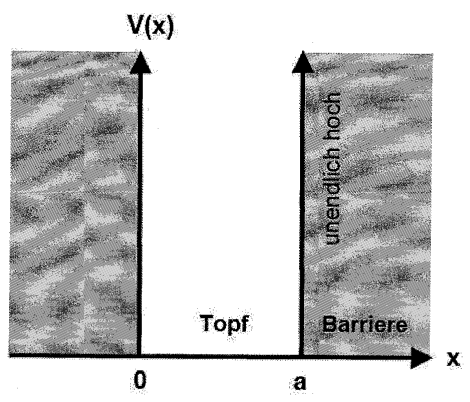
\includegraphics[width=0.3\textwidth]{fig/potentialtopf}
    \caption{Unendlich tiefer Potentialtopf}
    \label{fig:pottopf}
\end{figure}
Für die Schrödingergleichung
\begin{equation}
    \{-\frac{\hbar^2}{2m}\frac{\partial^2}{\partial x^2} \}\varphi(x) = E \varphi(x)
\end{equation}
Außerhalb des Topfes: $V(x) = \infty \rightarrow \varphi = 0$\\
Innterhalb des Topfes: $V(x) = 0$. Mit einfachem Lösungsansatz $\varphi (x) = A\cdot sin(kx)$ ergibt sich:
\begin{equation}
    E(k) = \hbar \omega = \frac{\hbar^2 k^2}{2m}
\end{equation}
Da die Lösung eine zusammenhängende Kurve sein muss muss an den Kanten des Topfes $\varphi(x=0) = \varphi(x=a) = 0$ gelten.
Durch den Sinus im Lösungsansatz ist links bereits $\varphi(x=0) = 0$, die rechte Seite kann mit $k = \frac{n\pi}{a}$ erfüllt werden.\\
Da $|\varphi(x)^2|$ der Wahrscheinlichkeit entspricht und diese über den ganzen Bereich $1$ ergeben muss, ergibt sich $A$ aus
der entsprechenden Normierung der Wellenfunktion:
\begin{equation}
    \int_{-\infty}^{+\infty} |\varphi(x)^2| dx = 1
\end{equation}
Und damit
\begin{equation}
    \varphi(x) = \frac{2}{a}sin(\frac{n\pi x}{a})
\end{equation}
\begin{equation}
    E_n = \frac{\hbar^2k_n^2}{2m} = \frac{\hbar^2\pi^2}{2ma^2}n^2
\end{equation}

\subsection{Tunnel-Effekt \todo{1x}}\label{k1:tunnEf}
\begin{enumerate}
    \item Barriere mit Potenzialschwelle in der Höhe von $V$ und mit der Breite $d$
    \item Teilchen mit Energie kleiner als $V$
    \item Klassische Mechanik: Teilchen wird \textit{immer} reflektiert
    \item Quantenmechanik: Teilchen durchdringt die Barriere mit einer gewissen Wahrscheinlichkeit (oder wird andernfalls relfektiert) $\rightarrow$ \textit{Es tunnelt}
\end{enumerate}
\begin{figure}
    \centering
    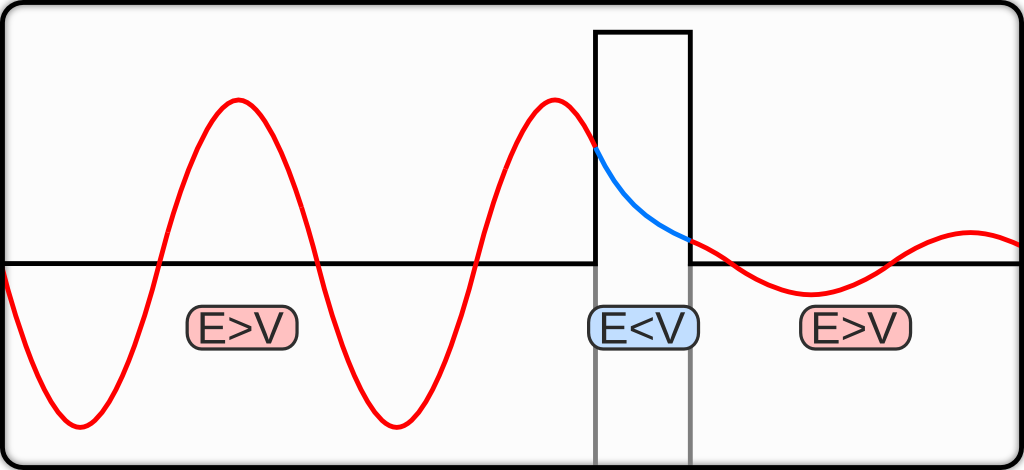
\includegraphics[width=0.66\textwidth]{fig/tunneleffektwiki.png}
    \caption{Schematische Darstellung des Tunneleffekts:
Ein Teilchen trifft von links kommend auf eine Potentialbarriere. Die Energie des getunnelten Teilchens bleibt gleich, nur die Amplitude der Wellenfunktion wird kleiner und somit die Wahrscheinlichkeit, das Teilchen aufzufinden.}
    \label{fig:tunneleffekt}
\end{figure}

Der Tunneleffekt wird für Dinge wie SRAM (Floating Gate MOS-FETs) und Rastertunnelmikroskope ausgenutzt. 

\subsubsection{Herleitung der Tunnelwahrscheinlichkeit}
Ist scheinbar noch nie gekommen, prinzipiell wird er über die zeitunabhängige (also stationäre) Schrödingergleichung angesetzt. 
Danach wird entlang der x-Achse zwischen drei Teilen unterschieden:
\begin{enumerate}
    \item I: Vor der Barriere, $V = 0$
    \begin{enumerate}
        \item Für die Wellenfunktion: $\varphi_I(x) = A_1e^{ikx} + A_2e^{-ikx}$ (Superposition von einer planaren nach rechts bzw. links laufenden Welle - die linke steht für den reflektierten Anteil)
    \end{enumerate}
    \item II: In der Barriere, $E > V \rightarrow E - V$ (Energie der Welle ist größer als die Barriere)
    \begin{enumerate}
        \item In der Barriere gibt es nicht wirklich eine Wellenfunktion, sondern einfach einen exponentiellen Verlauf, weswegen dort die komplexe Zahl im exponenten fehlt:
        \item $\varphi_{II}(x) = B_1e^{\kappa x} + B_2e^{-\kappa x}$
    \end{enumerate}
    \item III: Nach der Barriere $V = 0$ geht es weiter wie gewohnt
    \begin{enumerate}
        \item Nur neue Amplituden müssen wir einführen, da ja die Wahrscheinlichkeit eines Antreffens niedriger sein wird:
        \item $\varphi_{III}(x) = C_1e^{ikx} + C_2e^{-ikx}$
    \end{enumerate}
\end{enumerate}

Jetzt kann man einige Überlegungen für die Amplituden anstellen:
\begin{enumerate}
    \item $A_1$ und $A_2$ sind uns beide nicht bekannt, aber wir können mal normieren $A_1 = 1$
    \item $B_1$ und $B_2$ sind uns beide nicht bekannt
    \item $C_1$ ist die Welle die nach rechts läuft - die behalten wir! $C_2$ wäre der reflektierte Anteil, aber nach dem Tunneln gibt es keine Reflexion mehr, also gilt $C_2 = 0$
\end{enumerate}

%--------------------------------------------------------------------------------
%--------------------------------------------------------------------------------
%--------------------------------------------------------------------------------
\section{Periodische Festkörperstrukturen - Kapitel 2}
\subsection{Unterschied Halbleiter vs Metalle \todo{0x}}\label{k2:metalle}
Metalle: Gute Leitf\"ahigkeit aufgrund des vorhandenen Elektronengas. Bereits mit wenig Energie werden genug Elektronen gel\"ost um zu leiten.\\
Halbleiter: Leitf\"ahigkeit liegt zwischen Leitern und Nichtleitern. (Bandl\"ucke $< 1eV$)\\
Nichtleiter (Bandl\"ucke $> 3eV$).\\
Siehe \Cref{fig:bandLHL}.
\begin{figure}[h]
        \centering
        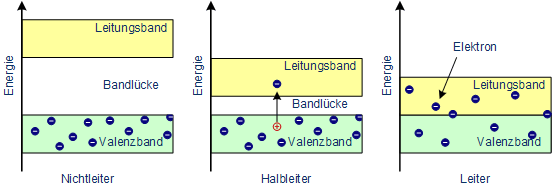
\includegraphics[width=0.6\textwidth]{fig/baendermodellLHL}
        \caption{B\"andermodell f\"ur Nichtleiter, Halbleiter und Leiter}
        \label{fig:bandLHL}
\end{figure}

\subsection{Grund für die Bildung von Festkörpern \todo{1x}}\label{k2:festkorper}
Ausgang: Wasserstoffatom als Modellsubstanz. Hier gillt eine sph\"arische Wellenfunktion:
\begin{equation}
    \Psi_H(r) = C \cdot e^{(-\frac{r}{a_0})}
\end{equation}
mit $a_0$ Bohr'scher Radius.\\
Daraus wird ein 2D-Gitter aus Automen gebaut, wobei davon ausgegangen wird dass Bindungen nur zwischen n\"achsten Nachbaren auftritt (tight binding Methode).
Die Energieskala wird so gew\"ahlt, dass der Zustand des neutralen Atoms (das Elektron befindet sich direkt am Atom) dem Energienullpunkt entspricht.\\
Gibt man einen weiteren Wasserstoffkern dazu, kann sich das Elektron entweder so positionieren, dass es beide Potentiale sp\"urt (seine Energie wird abgesenkt, $\Psi_1$, bindender Zustand) oder so, dass es sich nur bei den Ionen aufhält (seine Energie wird angehoben, $\Psi_2$, anti-bindender-Zustand).
\begin{center}
    \begin{align*}
        \Psi_1 &= \Psi_H(r_1)+\Psi_H(r_2)\\
        \Psi_2 &= \Psi_H(r_1)-\Psi_H(r_2)
    \end{align*}
\end{center}
\begin{figure}[h]
        \centering
        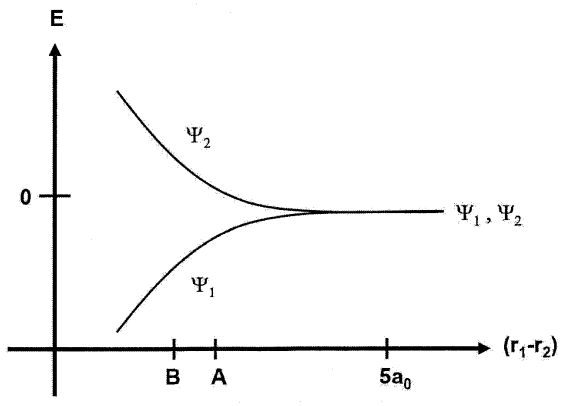
\includegraphics[width=0.6\textwidth]{fig/atomdistanz}
        \caption{Energie des bindenden- und anti-bindenden Zustands in Abh\"angigkeit vom Abstand der Atome. A = metall, B = halbleiter}
        \label{fig:atomdistanz}
\end{figure}
\subsection{Leitungsband, Valenzband, Ef aufzeichnen \todo{2x}}\label{k2:leitungsBand}

Siehe \Cref{fig:bandLHL}. Ef?

\subsection{Kroning Penny Modell \todo{0x}}\label{k2:kroningpenny}
Vereinfachtes Modell für Elektronen in Kristallgitter, verwendet ein einfaches periodisches Kristallpotenzial \autoref{fig:kronig-penney} ($a_0$ ist die Gitterkonstante)

\begin{equation}
    V(x + a_0) = V(x)
\end{equation}

\begin{figure}
    \centering
    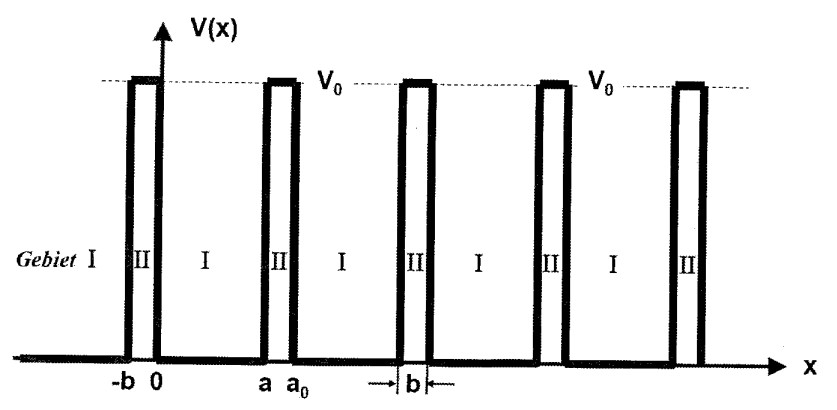
\includegraphics[width=0.66\textwidth]{fig/kronig-penny.jpg}
    \caption{Eindimensionales Kronig-Penney-Potenzial}
    \label{fig:kronig-penney}
\end{figure}

und vernachlässigt alle anderen Wechselwirkungen. Die Wellenfunktion der Elektronen sind Bloch-Funktionen.
Eine \textit{Bloch-Welle} (\autoref{fig:h-wave}) ist eine spezielle Wellenfunktion. Sie wird durch eine einfache planare Welle die mit einer periodische Funktion moduliert wird beschrieben.
Das schaut dann so aus:
\begin{equation}
    \Psi(r) = e^{i\cdot k\cdot r}\cdot u(r)
\end{equation}

\begin{figure}
    \centering
    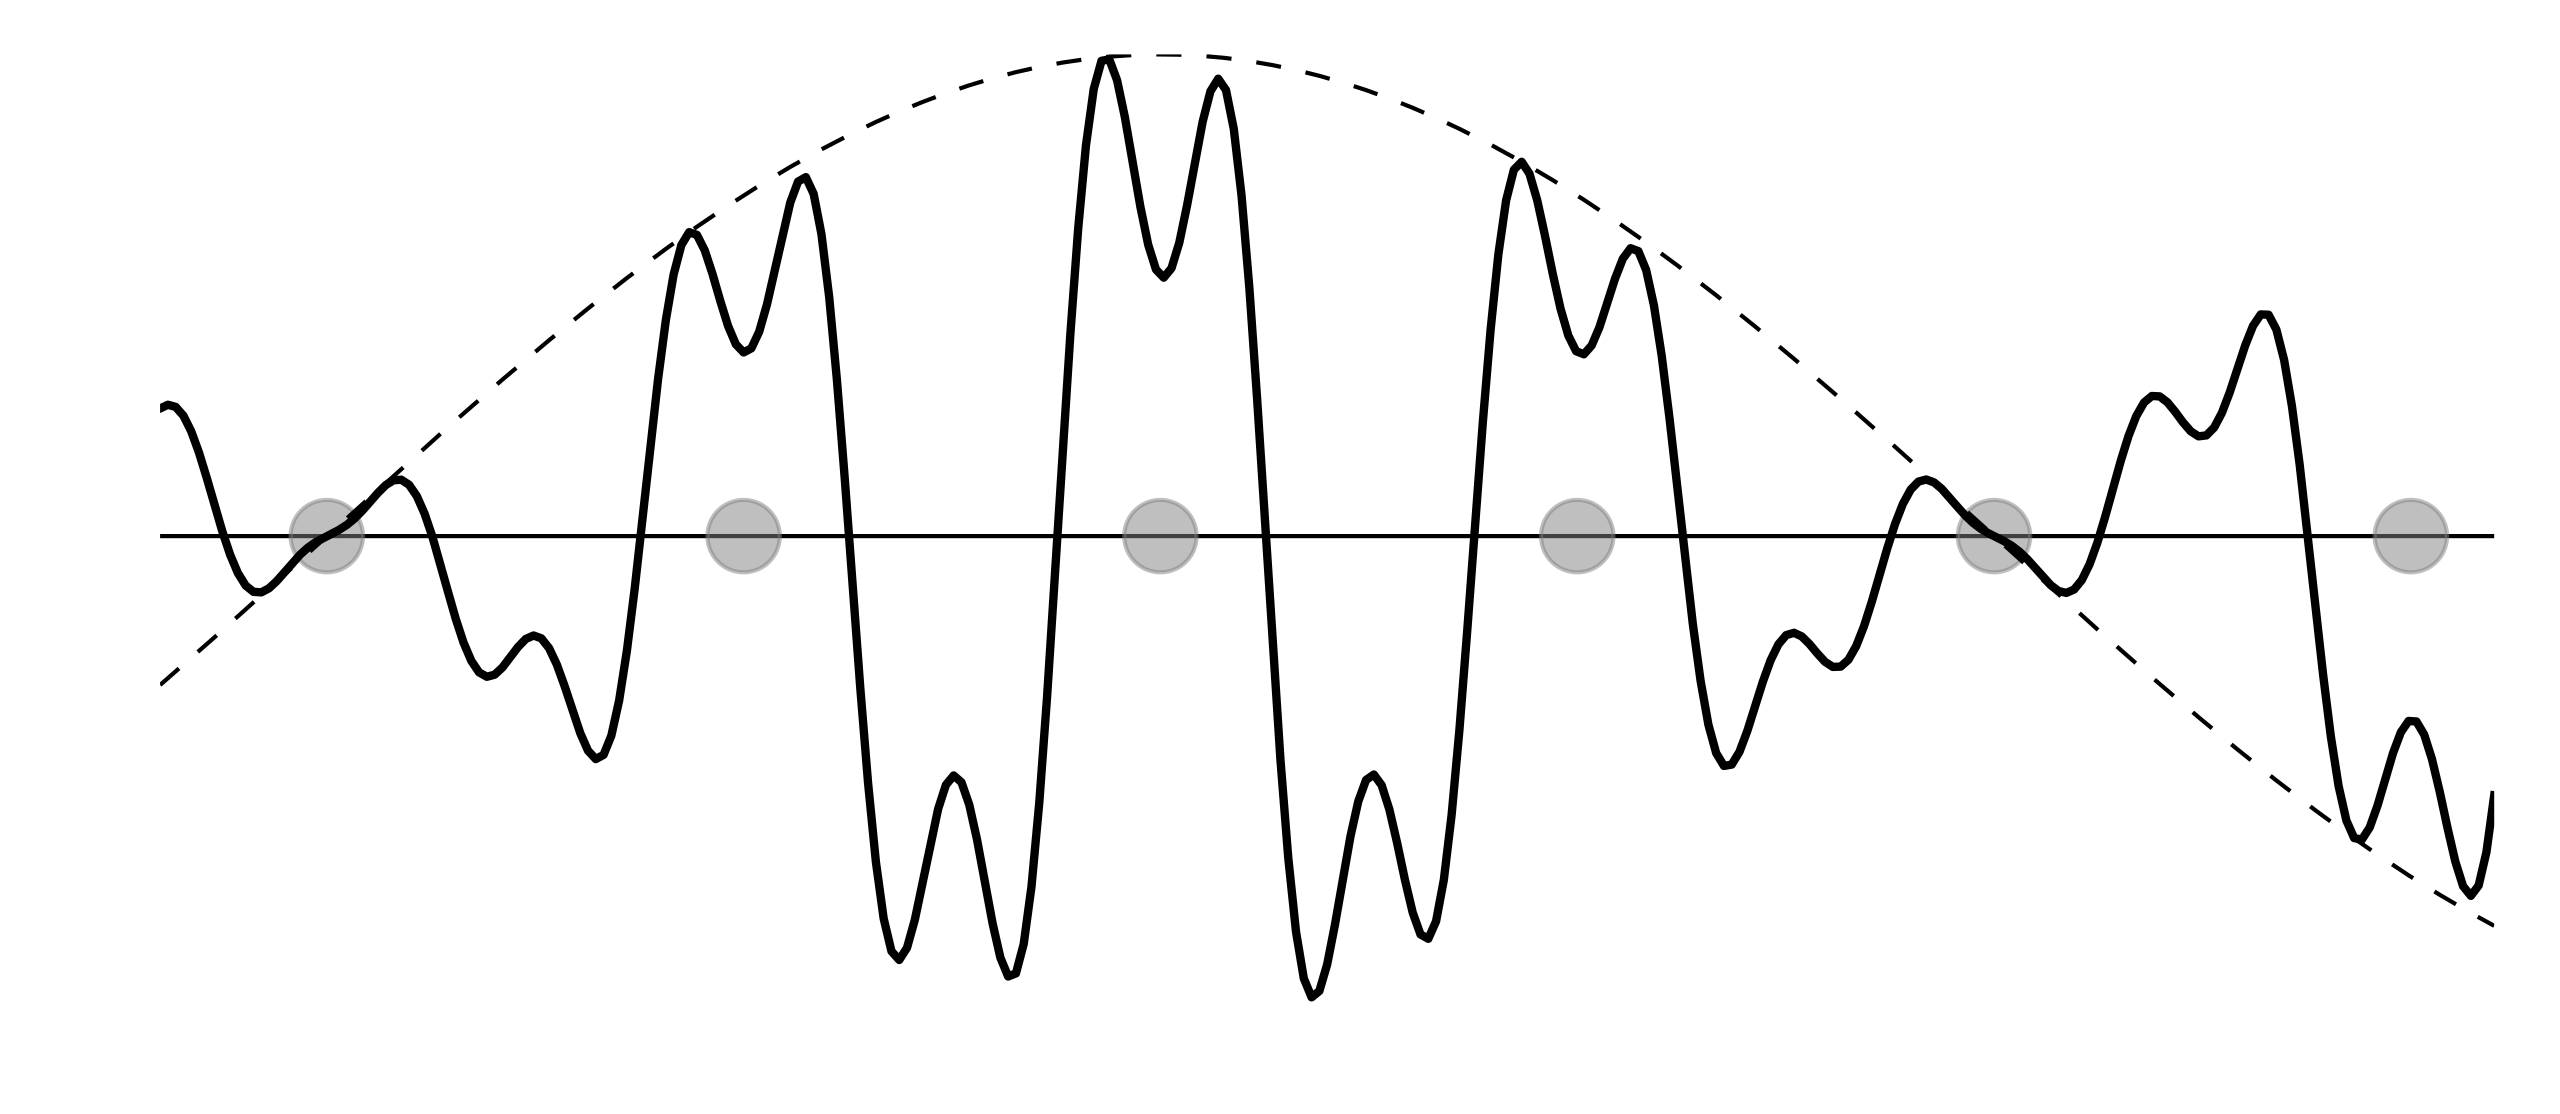
\includegraphics[width=0.66\textwidth]{fig/bloch-wave}
    \caption{Solid line: A schematic of a typical Bloch wave in one dimension. (The actual wave is complex; this is the real part.) The dotted line is from the $e^{ikr}$ factor. The light circles represent atoms.}
    \label{fig:h-wave}
\end{figure}

\begin{enumerate}
    \item $r$ ... Position
    \item $u$ ... periodische Funktion mit der selben periodizität wie das Kristallgitter
    \item $k$ ... Wellenvektor
\end{enumerate}

Herleitung für das eindimensionale Problem über periodische Kette von Rechteckbarrieren. Darüber kann man dann die Schrödinger Gleichung lösen, der Ansatz dafür ist folgender: $\Psi_k(x) = u_k(x)\cdot e^{ikx}$, wobei $u(x) = u(x+a+b)$ (Blochfunktion).

Man kann das Modell dann weiter vereinfachen (Breite Potenzialbarrieren gegen 0, Barrierenwirkung aber gleich) und es ergibt sich eine Bestimmungsgleichung  für die erlaubten Energiebänder für eine bestimmte Barrierestärke $P = \frac{ma}{\hbar^2} \cdot V_0 \cdot b$.

Die Bestimmungsgleichung selbst sieht so aus: 

\begin{equation}
    P\frac{sin(\alpha a)}{\alpha a} + cos(\alpha a) = cos(ka)
\end{equation}

Die Bestimmungsgleichung (auch Eigenwertgleichung) für die erlaubten Energiebänder enthält jetzt nur mehr die folgenden Paramter:

\begin{enumerate}
    \item P ... Barrierenstärke
    \item a ... Gitterkonstante (der Abstand zweier benachbarter Gitterelemente)
    \item $\alpha$ ... Indirekt die Energie
\end{enumerate}

\subsubsection{Grafische Lösung}
\begin{figure}
    \centering
    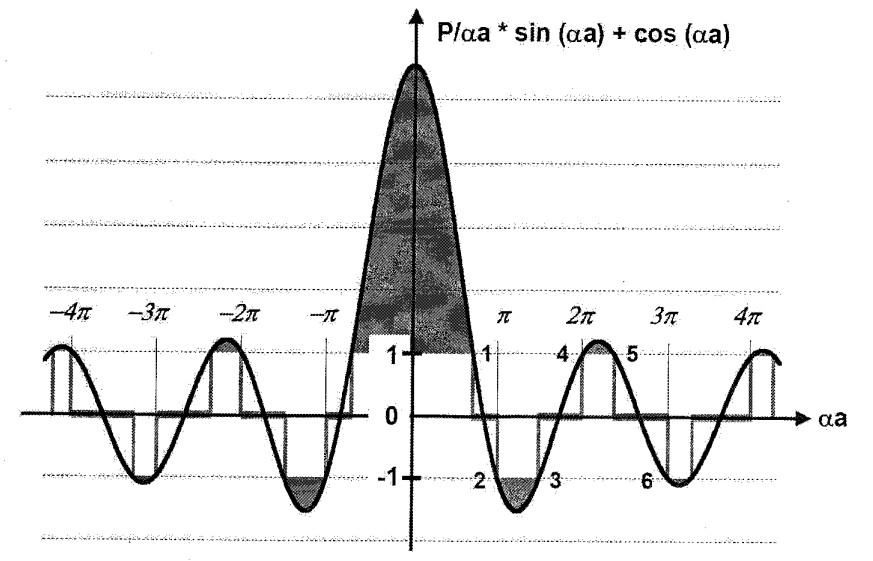
\includegraphics[width=0.66\textwidth]{fig/krong-penney-grafisch.jpg}
    \caption{Graphische Lösung des Kronig-Penney-Modells}
    \label{fig:kronig-penney-grafisch}
\end{figure}



Erkl\"aren, Skizzen, Rechenvorgang, grafische L\"osung, Herleitung e(k) Diagramm

\subsection{Entstehung der Halbleiter \todo{0x}}\label{k2:entstehungHalbleiter}

Verschiebt man die inneren Atome einer periodischen atomaren Anordnung so, dass der Abstand eines Paares kleiner wird als der Abstand der anderen Atome, \"andert sich die Verteilung der Energieniveaus. Die Bindungsenergie des n\"aheren Paares steigt, der Abstand zwischen bindendem und anti-bindendem Zustand wird wesentlich gr\"o{\ss}er. F\"ugt man weitere Atome hinzu, belibt der gr\"o{
\ss}ere Energieabstand erhalten. Die weiteren Energieniveaus gruppieren sich um die bindende und anti-bindende Energie (\Cref{fig:energieHalbleiter}).

\begin{figure}[h]
        \centering
        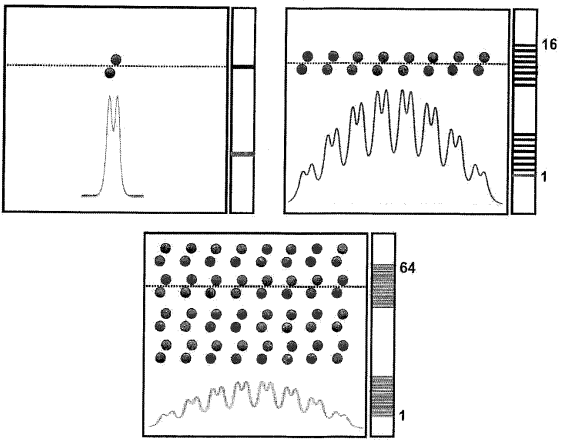
\includegraphics[width=0.6\textwidth]{fig/energieHalbleiter}
        \caption{Energiegruppierung in Halbleitern}
        \label{fig:energieHalbleiter}
\end{figure}

Es entstehen immer dann Halbleiter, wenn sowohl k\"urzere als auch l\"angere Bindungsl\"angen existieren. Erreichen kann man das z.B. durch inneinanderstellen von zwei Gittern (\Cref{fig:gitterstrukturen}).

\begin{figure}[h]
        \centering
        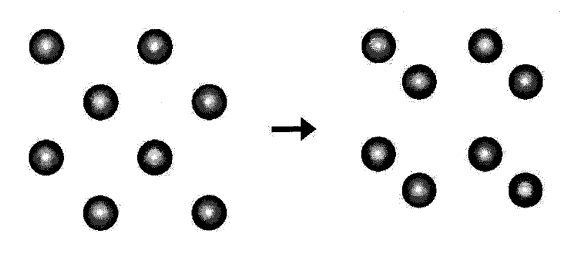
\includegraphics[width=0.6\textwidth]{fig/gitterstrukturen}
        \caption{Anordnung des zweidimensionalen Gitters}
        \label{fig:gitterstrukturen}
\end{figure}

Auf Grund der st\"arkeren Bindungen sind Halbleiter h\"arter als Metalle. Bei $T=0K$ haben sie keine Leitf\"ahigkeit.
Das untere Band (Name Valenzband) ist vollständig mit Elektronen besetzt, das obere Band (Leitungsband) ist leer.
Es gibt gleich viele Zustände im unteren und oberen Band. Wenn Ladungsträger ins obere Band angeregt werden, können
sie sich frei bewegen und führen zu einer hohen Leitfähigkeit.

\subsection{Phononen \todo{0x}}\label{k2:phononen}
F\"ur zwischenatomare Kr\"afte kann ein lineares Kraftgesetzt angenommen werden. Die Gitterschwingungen sind dann harmonische Oszillatoren mit quantisierter Energie $(n+\frac{1}{2}\hbar \omega)$.
Weil die m\"oglichen Energieniveaus einer Schwingung den gleichen Abstand $\hbar \omega$ besitzen, k\"onnen die Gitterschwingungen (analog zu den Photonen im elektrischen Feld) als teilchen gesehen werden, diese werden Phononen genannt. Sie geh\"oren zu den Bosonen.

\begin{table}[H]
    \centering
    \begin{tabular}{rcc}
         & Elektron & Phonon \\
         Ausbreitungsvektor & $\vec{k}$ & $\vec{q}$ \\
         Impuls & $\vec{p} = \hbar \cdot \vec{k}$ & $\vec{p} = \hbar \cdot \vec{q}$ 
    \end{tabular}
\end{table}

Bei Phononen spricht man vom Kristallimpuls, der nicht der Schwingung der Atome entspricht.\\
Die Zahl der im Mittel angeregten Phononen ist durch die Bose-Einstein Beziehung gegeben:
\begin{equation}
    n = \frac{1}{e^{\frac{\hbar\omega}{k_B T}}-1}
\end{equation}

%--------------------------------------------------------------------------------
%-------------------------o------------------------------------------------------
%--------------------------------------------------------------------------------
\section{Transporteffekte in Halbleitern - Kapitel 3}

\subsection{Berechnung der Diffusionsspannung \todo{1x}}\label{k3:diffusion}
Feldst\"arke (Poissongleichung) integrieren und die Skizzen von pn-\"Ubergang, elektrischer
Feldst\"arke und Spannungsverlauf.\\
Siehe \Cref{k5:rlz}.

\subsection{Alle Gleichungen (2x Stromgleichung, 2x Kontinuitätsgleichung, 1x Poisson-Gleichung) \todo{1x}}\label{k3:alleGleichungen}

\subsection{Dotieren \todo{0x}}\label{k3:dotieren}
Dotieren beschreibt den gezielten einbau von Fremdatomen um Ladungstr\"ager zu erzeugen, wodurch die Leitf\"ahigkeit eines
Halbleiters ver\"andert wird. Es kommt zu einer unterschiedlichen Konzentration aus Elektronen bzw. L\"ochern und es wird
nun von einem extrinsischem Halbleiter gesprochen.\\
Durch Dotierung werden Energieniveaus im verbotenen Band erzeugt. Ein Fremdatom aus der 5. Spalte des periodischen Systems
der Elemente wie z.B. P, As oder Sb erzeugt ein Energieniveau in der unmittelbaren Nachbarschaft der Unterkante $E_C$ des
Leitungsbandes. Dieses Energieniveau entsteht dadurch, dass das 5.Valenzelektron der äußersten Schale nicht an der
Bindung im Kristallgitter teilnimmt. Deshalb kann dieses Elektron bereits durch geringfügige Energiezufuhr vom oatierungsatom
abgelöst und in das Leitungsband gehoben werden, wo es sich als Leitungselektron frei bewegt.
Allerdings bleibt zufolge der Ablösung des negativen Elektrons am Dotieratom eine ortsfeste positive Ladung übrig. Die
Ladungen der Dotieratome können selbstverständlich nicht zum Stromtransport beitragen, spielen aber eine wichtige Rolle in
Halbleiterbauelementen.\\
Man nennt einen mit Akzeptoren dotierten Halbleiter kurz p-Halbleiter, den mit Donatoren dotierten n-Halbleiter.

\subsection{Verlauf der Ladungstr\"agerkonzentration als Funktion der Temperatur \todo{0x}}\label{k3:ladungstraegerkonz}
\Cref{fig:fermi}.

\begin{figure}[H]
    \centering
    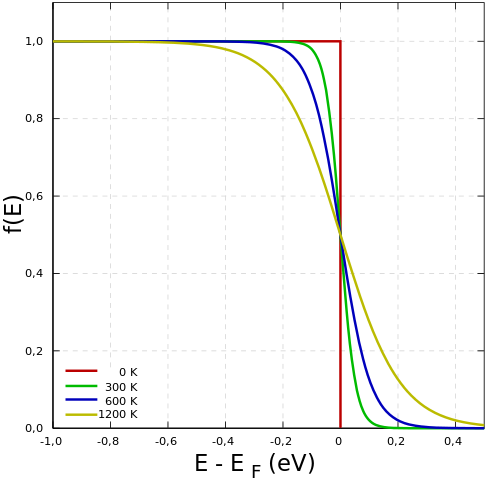
\includegraphics[width=0.4\textwidth]{fig/fermi}
    \caption{Ladungstr\"agerkonzentration bei verschiedenen Temperaturen (\Cref{fig:fermi})}
    \label{fig:fermi2}
\end{figure}

\subsection{Drude Modell \todo{0x}}\label{k3:drude}

Das Drude Modell ist eine klassische Beschreibung des Ladungstransports durch ein externes elektrisches Feld in Metallen.

Im Drude-Modell wird ein elektrischer Leiter als Ionenkristall betrachtet, in dem sich die Elektronen frei bewegen können, ein Elektronengas bilden und so verantwortlich für die Stromleitung sind. Der Begriff Elektronengas rührt von der Ähnlichkeit dieser Theorie zur kinetischen Gastheorie her: herrscht im Inneren des Leiters nämlich kein elektrisches Feld, so verhalten sich die Elektronen wie Gasteilchen in einem Behälter.

Durch ein äußeres elektrisches Feld $\vec {E}$ erfahren die freien Elektronen im Leiter eine Kraftwirkung $F_{el} = q \cdot E$ und werden beschleunigt, jedoch nicht kontinuierlich. Wäre dies so, dann dürften der Widerstand und die Stromstärke nicht konstant sein und das ohmsche Gesetz würde somit nicht gelten. Nach kurzer Zeit stellt sich jedoch ein Gleichgewicht ein, bei dem die mittlere Geschwindigkeit des Elektrons und damit der elektrische Strom proportional zur Feldstärke ist.

Dies wird vom Drude-Modell dadurch erklärt, dass das Elektron mit einem Gitterion zusammenstößt und abgebremst wird. Dieser Vorgang wird phänomenologisch durch eine mittlere Stoßzeit $\tau$ zwischen zwei Kollisionen beschrieben. Mit steigender Temperatur sinkt die mittlere Stoßzeit und damit auch die elektrische Leitfähigkeit der Metalle.

Die Bewegungsgleichung hierfür lautet:
\begin{equation}
    m \dot v + \frac{m}{\tau} v_D = -eE
\end{equation}
mit
\begin{itemize}
    \item $m$ der Elektronenmasse
    \item $v$ der Elektronengeschwindigkeit
    \item $v_D$ der Driftgeschwindigkeit (e-Geschwindigkeit abzüglich der thermischen Geschwindigkeit) und
    \item $\tau$ der Stoßzeit
    \item $e$ der Elementarladung.
\end{itemize}
Für den stationären Zustand $\dot v=0$ gilt:
\begin{equation}
    v_D = -\frac{e\cdot \tau}{m}E
\end{equation}
Mit der Ladungsträgerdichte $n$ n ergibt sich die Stromdichte $j$ damit zu:
\begin{equation}
    j = -e \cdot n \cdot v_D = \frac{e^2 \cdot \tau \cdot n}{m}E
\end{equation}
Die Leitfähigkeit $\sigma$ ist daher:
\begin{equation}
    \sigma = \frac{j}{E} = \frac{e^2 \cdot \tau \cdot n}{m}
\end{equation}

Diese Gleichung wird auch als Drude-Formel oder Drude-Leitfähigkeit bezeichnet. 

\subsection{Hall-Effekt \todo{0x}}\label{k3:halleffekt}
Metallplatte aufzeichnen mit Koordinatensystem und I, B, und F bzw. E als Vektoren.
Kurz beschreiben was im p-HL und n-HL passiert.
Erk\"aren warum der Strom nur in eine Richtung flie{\ss}en kann.

Hall Effekt wird verwendet um Magnetfelder oder Ladungsträgerart (Elektronen oder L\"ocher) und deren Dichte zu bestimmen.
Eine Metallplatte unter spannung wird in des Magnetfeld gestellt.
Das Magnetfeld bewirkt durch die Lorentzkraft eine ablekung der Elektronen senkrecht zur technischen Stromrichtung.
Es kommt zu einer Ladungstrennung (Elektronen und Löcher werden getrennt), die zu einem elektrischen Feld führt (entgegen der
Lorentzkraft). Die so entstandene Spannung lässt sich leicht abgreifen und dadurch kann man das Magnetfeld bestimmen
(\Cref{fig:hall}).

Die Hall-Spannung folgt Strom- und Magnetfeldänderungen in der Regel unmittelbar. Sie steigt mit dem Magnetfeld linear an und ist antiproportional zur (vorzeichenbehafteten) Ladungsträgerdichte[1], da eine geringere Anzahl von Ladungsträgern nur bei höherer Geschwindigkeit der Einzelladungen zu einer unveränderten Stromstärke führen kann. Auf die schnelleren Ladungsträger wirkt eine höhere Lorentz-Kraft, wodurch die Hall-Spannung größer wird. Da die Ladungsträgerdichte in Halbleitern bedeutend kleiner ist als in Metallen, werden vorwiegend Halbleiter als Hall-Sonden benutzt.

\begin{figure}[H]
    \centering
    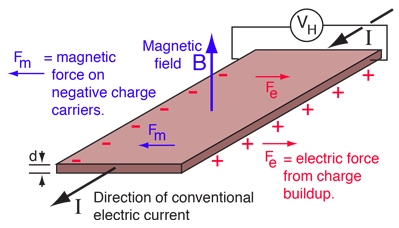
\includegraphics[width=0.4\textwidth]{fig/hall}
    \caption{Aufbau Hall-Effekt}
    \label{fig:hall}
\end{figure}

\subsection{Hall-Spannung \todo{0x}}\label{k3:hallspannung}

\subsection{Diffusionsstrom \todo{0x}}\label{k3:diffusionsstrom}

\subsection{Stromgleichungen \todo{0x}}\label{k3:stromgleichungen}

\subsection{Shockley-Haynes Experiment \todo{0x}}\label{k3:shockleyhaynes}
    \subsubsection{Schlatung aufzeichnen} Oszi und Spannungsquelle nicht vergessen
    \subsubsection{Kurve aufzeichnen und erkl\"aren was abgelesen werden kann}

\subsection{Kontinuit\"atsgleichungen \todo{0x}}\label{k3:kontinuitaet}

	\subsection{Intrinsische Ladungsträgerdichte $n_i$ + Gleichung $n \cdot p=n_i^2$ }
	Die intrinsische Ladungsträgerdichte beschreibt die Eigenleitungsdichte eines Halbleiters. Sie bestimmt den Mindestwert der elektrischen Leitfähigkeit.  
	Bei Halbleitern die auf den absoluten Nullpunkt gekühlt werden, sind alle Elektronen im Kristllgitter gebunden. Erst wenn die Temperatur erhöht wird, können Elektronen durch die nun zur Verfügung stehende thermische Energie vom Valenz- ins Leitungsband gehoben werden.
	Durch Rekombination wandern die Elektronen vom Leitungsband wieder ins Valenzband, dabei wird Energie freigesetzt. 
	Im thermodynamischen Gleichgewicht finden nun Rekombination und Generation von Elektronen statt. Diese sollten im Mittel gleich oft verkommen - um eben ein Gleichgewicht zu erhalten.
	Das bedeutet auch, dass die \textit{Anzahldichte} von freien Elektronen im Mittel konstant ist. 
	Die Eigenleitungsdichte $n_i$ setzt sich also aus der durchschnittlichen Anzahl an freien Elektronen $n$ und Löchern $p$ zusammen. Aufgrund des \textit{Massenwirkungsgesetzes}\footnote{Bei einer reversiblen Reaktion im chemischen Gleichgewicht hat der Quotient aus Ausgangsstoff (Elektron) und Reaktionsprodukt (Loch) einen festen charakteristischen Wert, auch Gleichgewichtskonstante genannt.} kann man schreiben:
	\begin{equation}
	    n_i^2 = n \cdot p
	\end{equation}
	Allerdings ist zu bedenken, dass sich die Eigenleitungsdichte massiv mit der Temperatur verändert, da durch die thermische Energie auch mehr Elektronen im Leitungsband zur Verfügung stehen - das ist auch der Grund warum dotierte Halbleiter ihre typischen Eigenschaften verlieren.
	Zum Beispielt verdoppelt sich $n_i$ bei einem Anstieg von 300 Kelvin auf 310 Kelvin.
	
	Diesen Effekt kann man über folgende Formel beschreiben:
	\begin{equation}
	    n_i^2 = n \cdot p = N_C \cdot N_V e^{-\frac{E_C-E_V}{kT}}
	\end{equation}\label{equ:eigenleitung}
	
	\begin{enumerate}
	    \item $N_C$ ... Bandgewicht des \emph{Leitungsbandes}, also die Zahl der Zustände in $\Delta E$ der Breite kT
	    \begin{enumerate}
	        \item Das Bandgewicht steigt mit der effektiven Masse und mit der Temperatur.
	        \item Höhere Temperatur bedeutet, dass mehr Zustände besetzt sind
	        \item Basiert auf der \textbf{Elektronendichte} $n$
	        \item Wikipedia nennt das die \textbf{Effektive Zustandsdichte} des Leitungsbands
	    \end{enumerate}
	    \item $N_V$ ... Bandgewicht des \emph{Valenzbandes}
	    \begin{enumerate}
	        \item Basiert auf der \textbf{Löcherdichte} $p$
	        \item Wikipedia nennt das die \textbf{Effektive Zustandsdichte} des Valenzbandes
	    \end{enumerate}
	    \item $E_C$ ... Energie der Unterkante des Leitungsbandes
	    \item $E_V$ ... Energie der Oberkante des Valenzbandes
	    \item $k$ ... Boltzmannkonstante
	\end{enumerate}
	
	\begin{enumerate}
	    \item Typische Größen für $n_i$ bei Raumtemperatur (26 Grad, 300 Kelvin)
	    \begin{enumerate}
	        \item Silizium: $1.5 \cdot 10^{10} cm^{-3}$
	        \item Germanium: $2.2 \cdot 10^{13} cm^{-3}$
	    \end{enumerate}
	\end{enumerate}
	
	\subsection{$n_i$ ist Funktion von was? (T und Gap)}
    Wie man in \autoref{equ:eigenleitung} sieht, ist die Eigenleitungsdichte $n_i$ von der Temperatur T abhängig.
    Die Temperaturabhängigkeit verringert sich wenn die Bandlücke, die sich aus $E_G = E_C - E_V$ ergibt, vergrößert. 
    
    Das macht Sinn, denn ein größerer Zähler aus \autoref{equ:eigenleitung} $e^{-\frac{E_G}{kT}}$ kaschiert Änderungen in der Temperatur besser.
    
    \subsubsection{Eigenleitung und Fermi-Niveau}
    Es soll noch erwähnt werden, dass die Eigenleitung $n_i^2$ auch zur Berechnung des Fermi-Niveaus herangezogen werden kann.
    Durch Lösen nach $n_i^2$ von \autoref{equ:eigenleitung} auf und einsetzen in andere Gleichungen kann man das Fermi-Niveau $E_F$ bestimmen bzw. auch zur Berechnung von \textit{p} und \textit{n} heranziehen. 
    Grundaussage ist aber, dass $E_F$ bei Eigenleitung in der Mitte des verbotenen Bandes liegt.
    

%--------------------------------------------------------------------------------
%--------------------------------------------------------------------------------
%--------------------------------------------------------------------------------
\section{Optische Eigenschaften von Halbleitern - Kapitel 4}

\subsection{Laser \todo{1x}}\label{k4:laser}
    \subsubsection{Wie funktionieren HL-Laser?}
    Licht kann von Halbleitern absorbiert und emittiert werden.
    Es gilt die Energieerhaltung: $\hbar \omega = \Delta E$, mit der Kreisfrequenz des absorbierten bzw. emittierten Lichts $\omega$,
    und der Energiedifferenz zwischen Anfangs- und Endzustand des Elektrons $\Delta E$.\\
    Es gibt
    \begin{enumerate}
        \item \emph{Interband\"uberg\"ange}, also \"Uberg\"ange zwischen zwei verschiedenen B\"andern
        \item \emph{Intraband\"uberg\"ange} innerhalb eines Bandes zwischen zwei verschiedenen Energieniveaus
    \end{enumerate}
    Die Wechselwirkung zwischen Elektronen und Photonen kann auf drei Arten geschehen:
    \begin{enumerate}
        \item \emph{Absorption}: Ein Photon mit der richtigen Energie kann in einem quanten-mechanischen System (mit einer gewissen Wahrscheinlichkeit) ein Elektron von einem niederenergetischen Zustand in einen höherenergetischen Zustand heben. Das Photon wird
        dabei vernichtet.
        \item \emph{Spontane Emission}: Ein Elektron in einem angeregten Zustand eines quanten-mechanischen Systems kann spontan ein Photon emittieren. Das Elektron fällt dabei vom höherenergetischen in den niederenergetischen Zustand. So funktionieren LEDs.
        \item \emph{Stimulierte Emission}: Trifft ein Photon auf ein angeregtes System, so kann (mit einer gewissen Wahrscheinlichkeit) ein zweites (identes) Photon erzeugt werden. Das Elektron fällt dabei vom höherenergetischen in den niederenergetischen Zustand.
        So funktionieren LASER (\textbf{L}ight \textbf{a}mplification by \textbf{s}timulated \textbf{e}mission of \textbf{r}adiaton).
    \end{enumerate}
    Beispielhafter Aufbau eines HL-Lasers in \Cref{fig:hlLaser}.
    \begin{figure}[H]
        \centering
        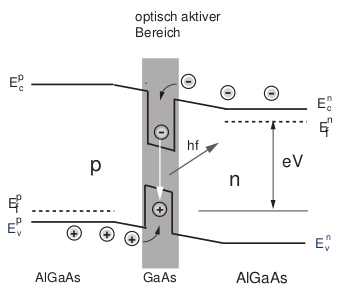
\includegraphics[width=0.6\textwidth]{fig/hlLaser}
        \caption{Aufbau eines HL-Lasers}
        \label{fig:hlLaser}
    \end{figure}
    Die Laserstrahlung liegt energetisch unter der Bandlücke des umgebenden Materials. Die Strahlung kann also problemlos aus dem Halbleiter heraus und wird nicht wieder absorbiert.
    \subsubsection{E(k) Diagramm}
        \begin{figure}[H]
            \centering
            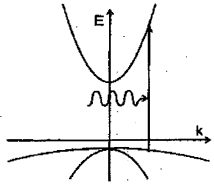
\includegraphics[width=0.3\textwidth]{fig/ekLaser}
            \caption{E(k)-Diagramm f\"ur Laser}
            \label{fig:ekLaser}
        \end{figure}
    \subsubsection{stimulierte Emission}
    Im thermodynamischen Gleichgewicht tritt stets Absorption auf ($Uv(E_1)-f_c(E_2) > 0$), nicht aber wenn der Halbleiter angeregt wird ($Uv(E_1)-f_c(E_2) < 0$), man spricht von Inversion.
    \subsubsection{Verst\"arkerbedingung}
    $E_{F_C}$ Fermi-Niveau Leitungsband\\
    $E_{F_V}$ Fermi-Niveau Valenzband\\
    Bedingung: $E_{F_C} - E_{F_V} > E_G$. ???\\
    Bei $T=0K$ genügt eine beliebig kleine Ladungsträgerinjektion, um die Quasi-Fermi-Niveaus $E_{F_c}$ und $E_{F_v}$ in die Bänder hinein zu verschieben (\Cref{fig:invLaser}) und die Verstärkerbedingung zu erfüllen. Bei Raumtemperatur ist allerdings eine relativ hohe Mindestladungsträgerdichte erforderlich, um Inversion zu erreichen ($ > 10^{18}/cm^3$).
        \begin{figure}[H]
            \centering
            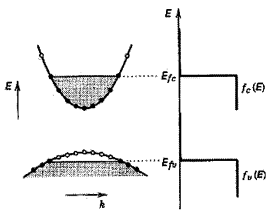
\includegraphics[width=0.3\textwidth]{fig/inversionLaser}
            \caption{Inversion bei $T=0K$}
            \label{fig:invLaser}
        \end{figure}

\subsection{Vergleiche direkte und indirekte Halbleiter \todo{1x}}\label{k4:inUndIndirekt}
    Bei direkten Halbleitern liegt das Maximum des Valenzbandes energetisch genau unter dem Minimum des Leitungsbandes, dies ist z.B. bei
    Galliumarsenid der Fall. Bei indirekten Halbleitern liegen diese ausgezeichneten Punkte bei unterschiedlichen k-Werten (Silizium, Germanium).
    \subsubsection{Wo ist k=0, was bedeutet das?}
    Beim direkten Halbleiter ist $k=0$ dort, wo das minimum des Leitungsbandes und das maximum des Valenzbandes liegen. Sonst???
    \subsubsection{w(k) für freies Teilchen}
    ???
    \subsubsection{Bewegt sich ein e- im Ev bei T=0?}
    ?\\
    Nein, bei $0K$ ist das Valenzband voll besetzt. Elektronen k\"onnen sich nirgends hin bewegen.
    \subsubsection{Wo ist die Masse am größten (Ev, Ec)?}
    ???
    \subsubsection{Gleichung für m*}
    Aufgrund der Auswirkung der Bandstruktur auf die Elektronen im Kristall scheinen diese dort eine andere Masse zu haben, sie wird
    effektive Masse $m^{*}$ genannt.
    \begin{equation}
        \frac{1}{m^{*}} = \frac{1}{\hbar^2}*\frac{d^2E}{dk^2}
    \end{equation}
    \begin{figure}
        \centering
        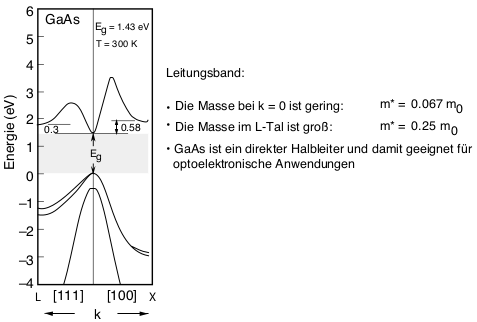
\includegraphics[width=0.8\textwidth]{fig/bandstrukturGaAs}
        \caption{Bandstruktur GaAs}
        \label{fig:bandGaAs}
    \end{figure}
    Betrachtet man die Bandstruktur von z.B. GaAs (\Cref{fig:bandGaAs}), erkennt man dass bei den Wendepunkten die Masse ins unendliche
    gehen w\"urde. Dies passiert aber nicht, in diesen Gebieten braucht es ein anderes Modell, die kp-Theorie.
    Am oberen Rand wird die effektive Masse negativ. Man spricht von einem Loch, die Ladung wird positiv.

\subsection{Zustandsdichte und Besetzungswahrscheinlichkeit \todo{2x}}\label{k4:zustandsDichte}
    Quantensysteme haben diskrete Zust\"ande.
    Die Zustandsdichte $g(E) = \frac{N}{L^3}$ gibt an wie viele Zust\"ande pro eV es zu einem gewissen Energieniveau gibt (Mit $N$ anzahl diskreter Zust\"ande, $L^3$ Volumen des HL).
    Die Besetzungswahrscheinlichkeit, auch Fermi-Verteilung, $P(E)$ gibt die Wahrscheinlichkeit an dass ein Zustand eingenommen wurde.
    Daraus l\"asst sich berechnen, wie viele Leitungstr\"ager vorhanden sind: $n = \int{g(E)*P(E) dE}$
    
    \subsubsection{Banddiagramme}
    ???
    \subsubsection{Temperaturabh\"angigkeit}
    Die Fermi-Verteilung ist Temperaturabh\"angig. Desto nidriger die Temperatur, desto steiler f\"allt die Verteilung ab.
    \begin{figure}[H]
        \centering
        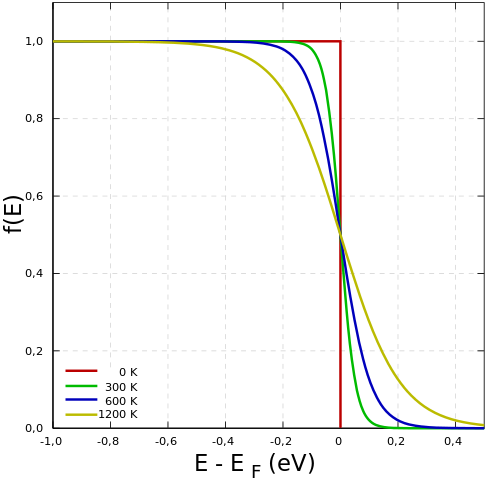
\includegraphics[width=0.5\textwidth]{fig/fermi}
        \caption{Fermi-Verteilung}
        \label{fig:fermi}
    \end{figure}

%--------------------------------------------------------------------------------
%--------------------------------------------------------------------------------
%--------------------------------------------------------------------------------
\section{Halbleiterdioden - Kapitel 5}

\subsection{PN-Übergang \todo{5x}}\label{k5:pn}
    
    \subsubsection{Raumladungszone}
	Elektronen aus dem \textit{n}-dotierten Bereich diffundieren zum \textit{p}-dotierten Bereich was zu einer Elektronenverarmung der \textit{n}-seitigen Randzone führt. 
	Dadurch wird die \textit{n} Seite positiv aufgeladen. Umgekehrt kommt es zu einer Löcherverarmung auf der \textit{p} Seite und somit zu einer negativen Aufladung dort. 
    Dadurch entsteht am Übergang eine hochohmige Verarmungszone, die sogenannte \textit{Raumladungszone} (RLZ).
    Diese Raumladung erzeugt ein Feld, welches der weiteren Diffusion von Ladungsträgern entgegenwirkt. Das Maximum der elektrischen Feldstärke liegt an der \textit{pn}-Grenze (\ref{fig:raumladungszone} b).
    
    Durch dieses elektrische Feld entsteht eine Potenzialdifferenz welche auch als \textit{Diffusionsspannung} bezeichnet wird berechnet sich folgendermaßen berechnet:
    \begin{equation}
        U_D = \varphi_2 - \varphi_1 = \int{x_1}^{x_2} E \cdot dx
    \end{equation}

           \begin{figure}[H]
        \centering
        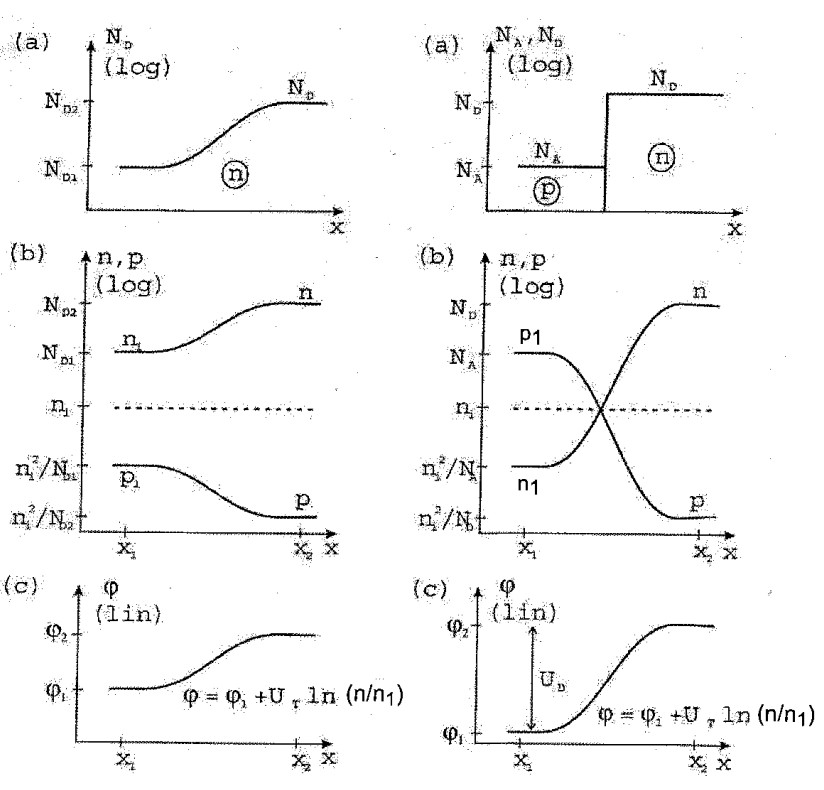
\includegraphics[width=0.5\textwidth]{fig/pnuebergang.jpg}
        \caption{linkes Bild: $nn^+$ -Übergang. Rechtes Bild: \textit{pn}-Übergang. (a) Dotierung (b) Ladungsträgerdichten (c) Potenzialverlauf}
        \label{fig:pnuebergang}
    \end{figure}
    
	$U_D$ in Silizium bei Zimmertemperatur beträgt ca. 0.8V 
    \begin{figure}[H]
        \centering
        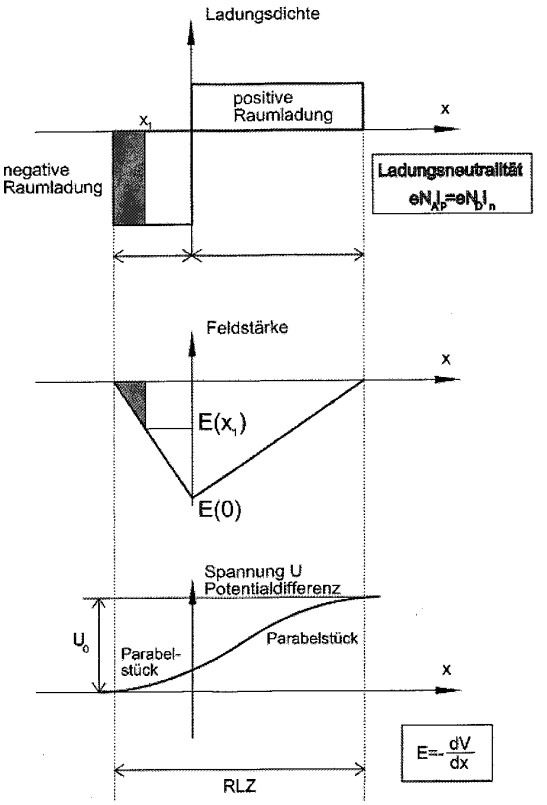
\includegraphics[width=0.5\textwidth]{fig/raumladungszone}
        \caption{Raumladungsdichte (a), Feldstärke (b) und Potenzial (c) am \textit{pn}-Übergang}
        \label{fig:raumladungszone}
    \end{figure}
    
       \begin{figure}[H]
        \centering
        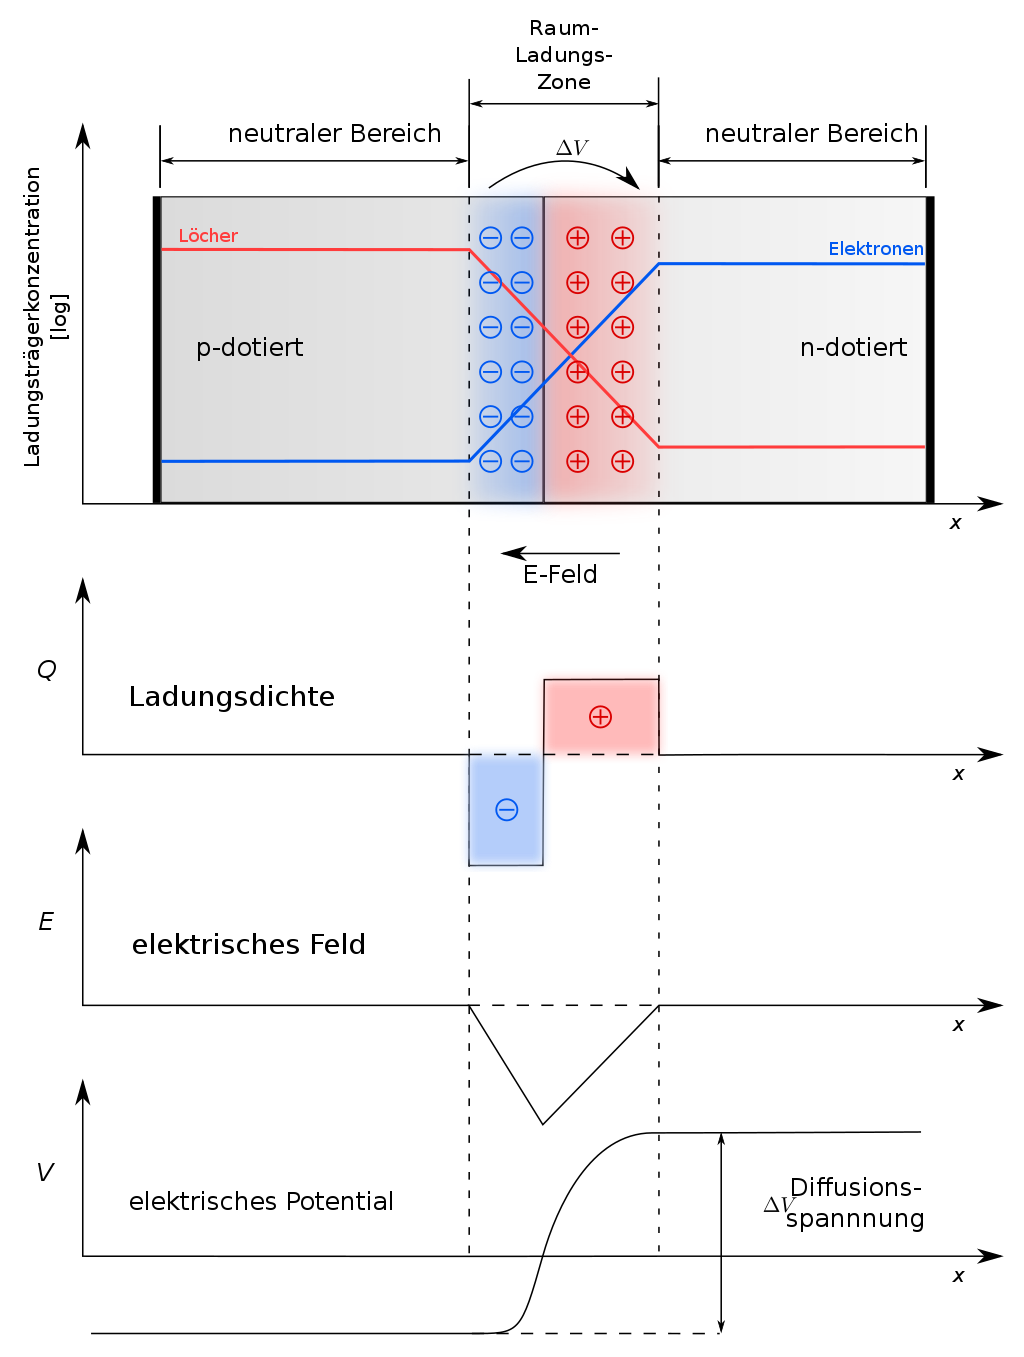
\includegraphics[width=0.5\textwidth]{fig/raumladungszone-wiki}
        \caption{Nochmal die Raumladungszone, diesmal von Wikipedia in Bunt und Farbe}
        \label{fig:raumladungszone-wiki}
    \end{figure}


	\subsubsection{Aufzeichnen ohne externe Spannung}
	Läuft wohl auf das darstellen der Raumladungszone und des elektrischen Feldes wie in \autoref{fig:raumladungszone-wiki} und \autoref{fig:raumladungszone} hinaus?
	Ohne externe Spannung kommt es wie oben beschrieben zur Ausbildung einer Raumladungszone. Bei dieser wandern die Elektronen aus dem n-Halbleiter zu den Löchern des p-Halbleiters und umgekehrt. Dabei entsteht eine Zone ohne freie Ladungsträger - eben die Raumladungszone. 
	
	\subsubsection{Diagramm dazu, wo auf x-Achse Ort (Verlauf von pn Übergang) und auf der y-Achse Dichte der freien Elektronen}
       \begin{figure}[H]
        \centering
        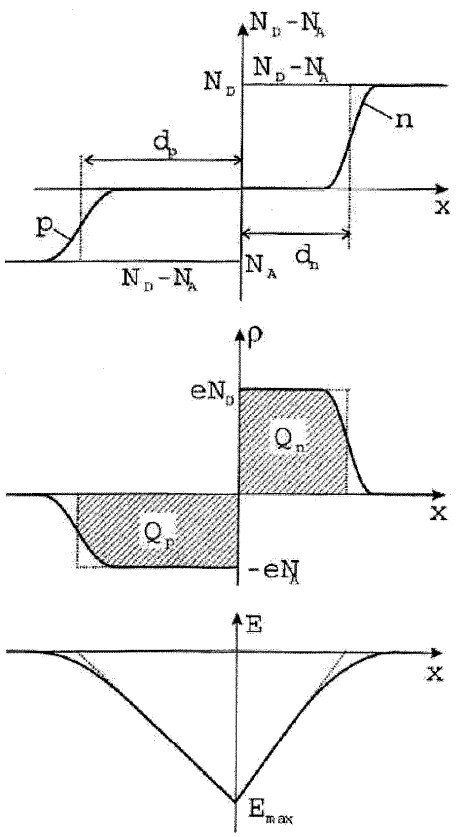
\includegraphics[width=0.5\textwidth]{fig/dotierungsVerlauf}
        \caption{Verlauf der Dotierung, der Trägerdichten \textit{n} und \textit{p}, der Raumladung $\rho$ und der Feldstärke E am abrupten \textit{pn}-Übergang. Beachten Sie, dass hier die Dichten linear aufgetragen sind.}
        \label{fig:dotierungsVerlauf}
    \end{figure}

	Hier kann man entweder mit \autoref{fig:raumladungszone-wiki} und \autoref{fig:raumladungszone} beginnen.
	Mehr Sinn macht es aber wahrscheinlich \autoref{fig:pnuebergang} aufzuzeichnen, oder sich auf \autoref{fig:dotierungsVerlauf} zu beziehen. 
	Dort kann man mit der Dotierung beginnen (diskreter Sprung, da p und n dotiert!) und die zweite Reihe stellt dann die Ladungsträgerdichte dar. Achtung, die Dichten sind logarithmisch angegeben!
	
	$N_A$ (p-Halbleiter) und $N_D$ (n-Halbleiter) stellen jeweils die Dotierungen dar, der Sprung stellt den Dotierungsverlauf / Übergang von p auf n dar.
	$n_i$ wird \textit{Intrinsic}-Zahl oder auch Eigenleitungsdichte genannt und beschreibt die Trägerdichte im undotierten Halbleiter und wird detailliert in Kapitel 3 diskutiert bzw. eingeführt. 
	
	Wikipedia hat dazu folgende Definition: Die Eigenleitungsdichte ist die charakterisierende Materialeigenschaft eines Halbleiters mit Blick auf seine elektrische Leitfähigkeit.
	Die Eigenleitungsdichte beschreibt den Mindestwert der elektrischen Leitfähigkeit, die tatsächliche Leitfähigkeit kann höher liegen (durch Verunreinigung, Dotierung). Diese Störstellenleitung (eben durch Dotierung) liegt üblicherweise um mehrere Größenordnungen über der Eigenleitung. 
	
	\subsubsection{Größenordnung einschätzen: Abstand von Elektronen, Größe von RLZ (normaler PN Übergang, Tunneldiode), Elektronendichte im HL}
	Ist eventuell in Kapitel 3 besprochen?
	
	\subsubsection{Skizze Flussrichtung, Sperrichtung, Raumladungszone}
	
	Wahrscheinlich ist hier die Darstellung des Bänderdiagramms gemeint, diese ist in \autoref{fig:pn-betriebszustände2}
	
       \begin{figure}[H]
        \centering
        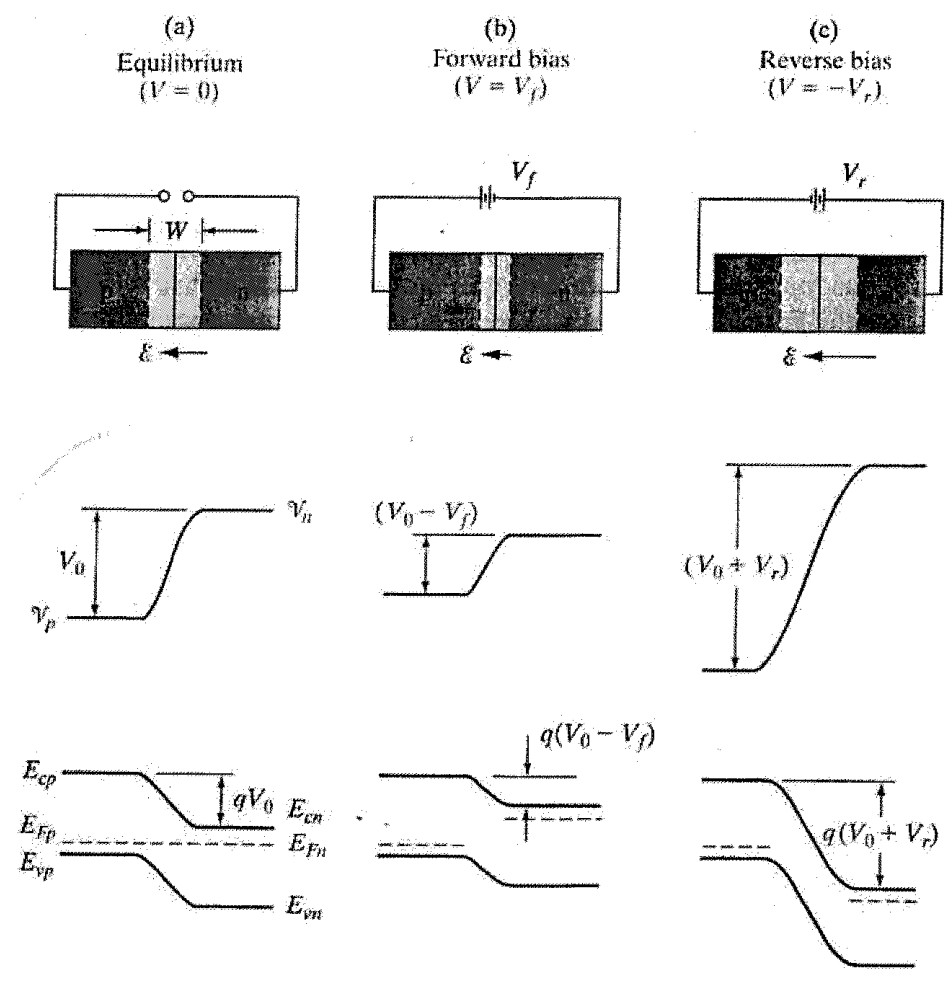
\includegraphics[width=0.5\textwidth]{fig/pn-fluss-sperr-rlz.jpg}
        \caption{Betriebszustände des pn-Übergangs (a) $U = 0$ (b) Flussrichtung $U = V_f$ (c) Sperrpolung $U = -V_r$, p-Zone negativ gegenüber n-Zone}
        \label{fig:pn-betriebszustände2}
    \end{figure}
	
    
       \begin{figure}[H]
        \centering
        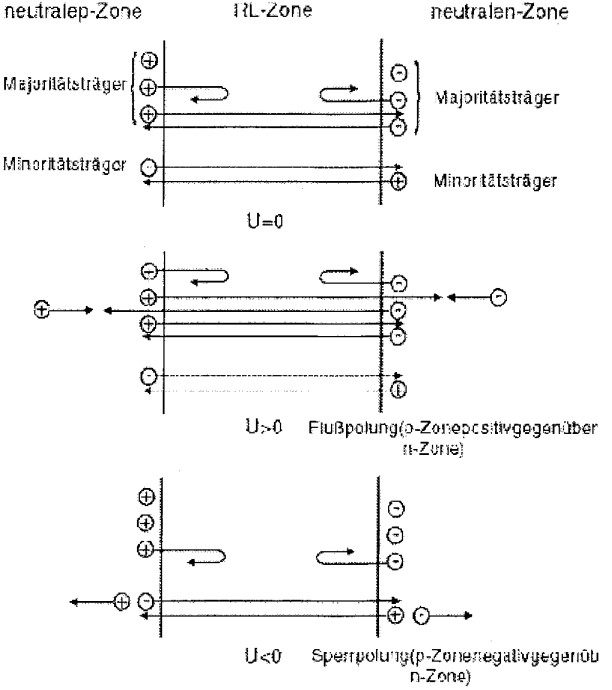
\includegraphics[width=0.5\textwidth]{fig/pn-betriebszustande}
        \caption{Betriebszustände des pn-Übergangs (oben) $U = 0$ (mitte) Flußpolung $U > 0$, p-Zone positiv gegenüber n-Zone (unten) Sperrpolung $U < 0$, p-Zone negativ gegenüber n-Zone}
        \label{fig:pn-betriebszustände}
    \end{figure}
    
    \subsubsection{Flussbetrieb}
    \emph{Noch einfachere Beschreibung (und korrekte)}: Bei Polung in Durchlassrichtung (+ am p-Kristall und - am n-Kristall) wird der Potentialwall abgebaut. Das elektrische Feld der Sperrschicht wird aber einer gewissen angelegten Spannun gkomplett neutralisiert und es ergibt sich mit dem von außen angelegten elktrischen Feld ein neues elektrisches Feld, welches Ladungstransport durch den gesamten Kristall erlaubt. Neue Ladungsträger fließen von der äußeren Quelle auf die Sperrschicht zu und rekombinieren hier fortwährend. Bei ausreichender angelegter Spannung fließein signifikanter elektrischer Strom.
    Das Skriptum hat dazu noch \autoref{fig:pn-flussbetrieb} zu bieten.
    
    \emph{Vereinfachte Beschreibung}: Legt man eine äußere Spannung U an, sodass das p-Gebiet gegenüber dem n-Gebiet positiver wird, so werden die Löcher auf die n-Seite und die Elektronen auf die p-Seite getrieben.
    
    \emph{Korrekte Beschreibung}: Die äußere Spannung U kann wegen der hohen Ladungsträgerdichten in den neutralen Zonen nur in der Raumladungszone abfallen. Sie verringert dort die Diffusionsspannung von $U_D$ (in Silizium 0.7V) auf $U_D-U$. 
    
    Elektronen und Löcher können nun wieder vermehrt durch Diffusion zur pn-Grenze wandern. Die Raumaldungszone wird mit beweglichen Ladungsträgern zugeschüttet und die Diode leitet. 
    
    Wegen der Verringerung der Potentialbarriere und des exponentiellen Verlaufes der Energieverteilung der Elektronen kommt es zu einer exponentiellen Abhängigkeit des Stromes von der Spannung (Exponentialkennlinie).
    
    \begin{figure}
        \centering
        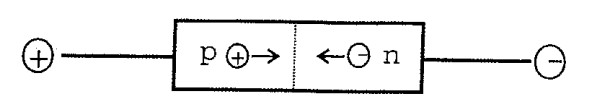
\includegraphics[width=0.33\textwidth]{fig/pn-flussbetrieb.jpg}
        \caption{Schematische Darstellung des Flussbetriebs}
        \label{fig:pn-flussbetrieb}
    \end{figure}
    
    \subsubsection{Sperrterieb}
    Durch Anlegen einer äußeren Spannung in Sperrichtung (+ am n-Kristall, - am p-Kristall) wird das elektrische Feld der Sperrschicht verstärkt und die Ausdehnung der Raumladungszone vergrößert. Elektronen und Löcher werden von der Sperrschicht weggezogen. Es fließt nur ein sehr geringer Strom, erzeugt durch Minoritätsladungsträger (Sperrstrom), außer die Durchbruchspannung wird überschritten.
    Aus dem Skriptum wieder: \autoref{fig:pn-sperrbetrieb}
    \begin{figure}
        \centering
        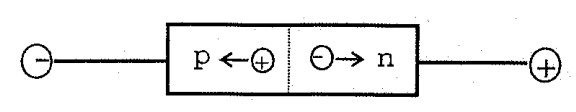
\includegraphics[width=0.33\textwidth]{fig/pn-sperrbetrieb.jpg}
        \caption{Schematische Darstellung des Sperrbetriebs}
        \label{fig:pn-sperrbetrieb}
    \end{figure}

	\subsubsection{Skalen, logarithmisch, linear, Größenordnung}
	\autoref{fig:dotierungsVerlauf} stellt die Raumladungszone linear dar, während \autoref{fig:pnuebergang} mit einer logarithmischen Darstellung arbeitet.
	Größenordungen werden wahrscheinlich wieder in Kapitel 3 erwähnt. 
	
	\subsubsection{Freie Elektronen}
	
	\subsubsection{Anzahl}
	\subsubsection{Dotierung}
	

	
\subsection{Diodenkennlinie \todo{0x}}\label{k5:diode}
Durch die Polung in Durchlassrichtung treibt die äußere Spannung sowohl die Elektronen aus dem n-Gebiet, als auch die Löcher aus dem p-Gebiet auf die Raumladungszone zu, die somit wieder bewegliche Ladungsträger enthält und ihre Sperrwirkung verliert. 
    \begin{figure}[H]
        \centering
        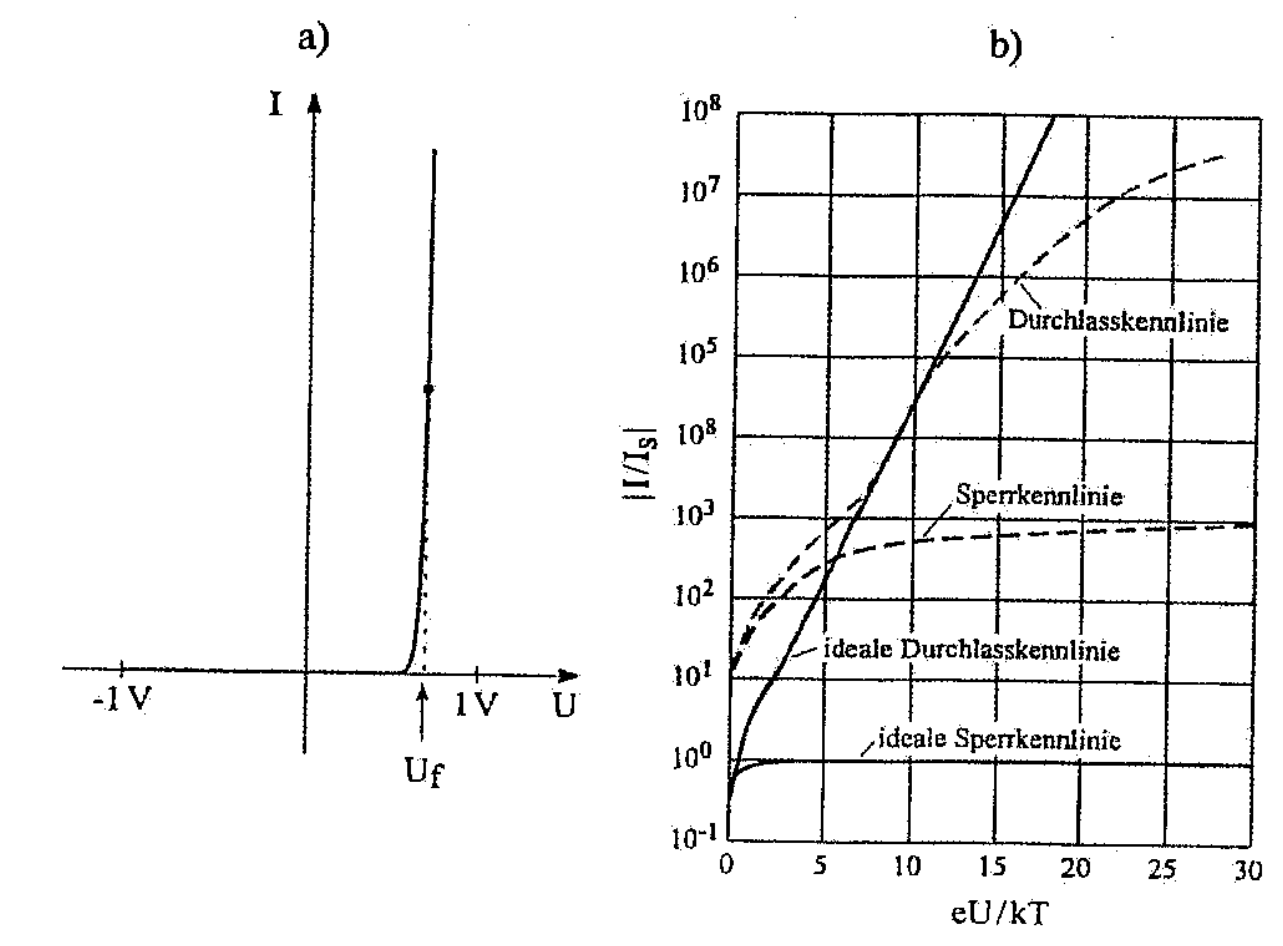
\includegraphics[width=0.8\textwidth]{fig/diodenkennlinie}
        \caption{(a) ideale Diodenkennlinie (linear), (b) ideale und nichtideale Kennlinie (logarithmisch)}
        \label{fig:diodenkennlinie}
    \end{figure}
    \subsubsection{Warum exponentiell?}
    Shockley-Gleichung in 2 Schritten:
    \begin{enumerate}
        \item Elektronenkonzentration am p-seitigen Rand der RLZ berechnen ( = L\"ocherkonzentration am p-seitigen Rand)
        \item Diffusion der Elektronen im neutralen p-Gebiet behandeln
    \end{enumerate}
    \begin{equation}
        I = I_S (e^{\frac{U_D}{n \cdot U_T}} - 1)
    \end{equation}
    Mit
    \begin{itemize}
        \item S\"attigungssperrstrom $I_S \approx 10^{-12} \ldots 10^{-6}A$
        \item Emissionskoeffizient $n \approx 1 \ldots 2$
        \item Temperaturspannung $U_T=\frac{k \cdot T}{q} \approx 25mV$ bei Raumtemperatur
        \item Temperatur $T$
        \item Boltzmannkonstante $k=1.381\cdot 10^{-23} Ws/K$
        \item Elementarladung $q = 1.602 \cdot 10^{-19}As$
    \end{itemize}
    \subsubsection{Verlauf der Kapazit\"at einer Diode als Funktion der Spannung}
    Der p-n \"Ubergang von Dioden hat eine Kapazit\"at, die von der Breite der RLZ abh\"angig ist. Mit steigender Sperrspannung vergr\"o{\ss}ert sich die Breite der ladungsfreien Zone, wodurch die Kapazit\"at abnimmt. Zu sehen in \Cref{fig:diodenkapazitaet} mit $m_s$ als Kapazit\"atskoeffizient, der das Dotierungsprofil darstellt.
    \begin{figure}
        \centering
        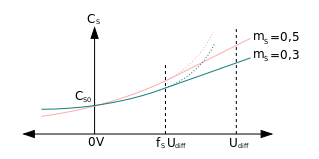
\includegraphics[width=0.5\textwidth]{fig/diodenkapazitaet}
        \caption{Sperrschichtkapazit\"at von Dioden}
        \label{fig:diodenkapazitaet}
    \end{figure}
    \subsubsection{Wie sehen die Ladungen bei anlegen einer Spannung aus?}
    Durch anlegen einer Spannung in Durchlassrichtung werden elektronen (aus dem n-Gebiet) und L\"ocher (aus dem p-Gebiet) in die RLZ getrieben. Die RLZ verschwindet und die Diode leitet.\\
    Bei anlegen einer Spannung in Sperrrichtung werden die Elektronen und L\"ocher noch weiter auseinandergetrieben, die RLZ wird gr\"o{\ss}er, die Diode sperrt.
    \subsubsection{Massenwirkungsgesetz}
    Siehe \Cref{k3:kontinuitaet}.

\subsection{Banddiagramm für PN ohne Spannung \todo{1x}}\label{k5:pnBand}
\begin{figure}
    \centering
    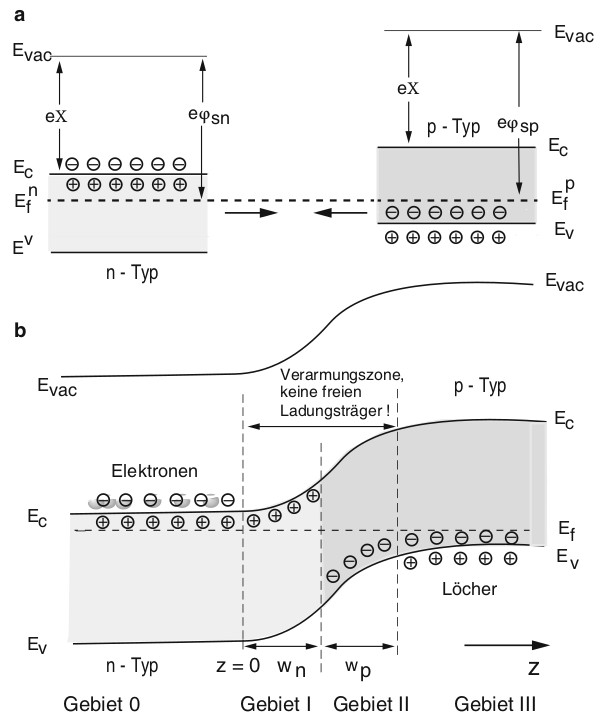
\includegraphics[width=0.66\textwidth]{fig/pn-bandstruktur.jpg}
    \caption{Formation eines pn-Übergangs. a Die p- und n-Gebiete vor der Formation des Über-
gangs. Im p-Gebiet liegt das Fermi-Niveau knapp oberhalb der Valenzbandkante, im n-Gebiet
knapp unterhalb des Leitungsbandes. Die Elektronenaffinitäten $e_\xi$ und Austrittsarbeiten $e\Phi_{sp}$
und $e\Phi_{sn}$ , sowie das Fermi-Niveau sind ebenfalls eingezeichnet. b Bandprofil des fertigen
pn-Übergangs inklusive Vakuumniveau. Die Bandlücke ist überall die gleiche und, wichtig, Va-
lenzband und Leitungsband verlaufen immer parallel.}
    \label{fig:pn-banddiagramm}
\end{figure}

\begin{figure}
    \centering
    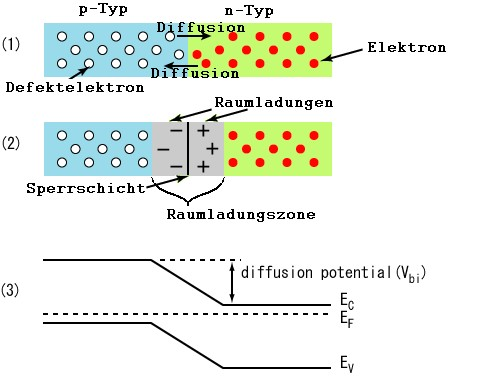
\includegraphics[width=0.66\textwidth]{fig/pn-banddiagramm2}
    \caption{Nochmal die selbe Darstellung mit bereits zusammengefügtem PN-Übergang.}
    \label{fig:pn-banddiagramm}
\end{figure}



\subsection{Tunneleffekt \todo{1x}}\label{k5:tunnelEffekt}
    \subsubsection{Flussspannung}
    \subsubsection{Energieerhaltung}
    \subsubsection{Endliche Barriere}
    \subsubsection{Einfaches Tunneln}

\subsection{Schottky-Kontakt-Diode \todo{0x}}\label{k5:schottky}
Schottky-Dioden werden aus einem Metall-Halbleiter Kontakt gebaut. Dies geschieht implizit bei jedem Kontakt von Transistoren und Dioden und hat dementsprechend hohe Wichtigkeit.

\begin{figure}[h]
    \centering
    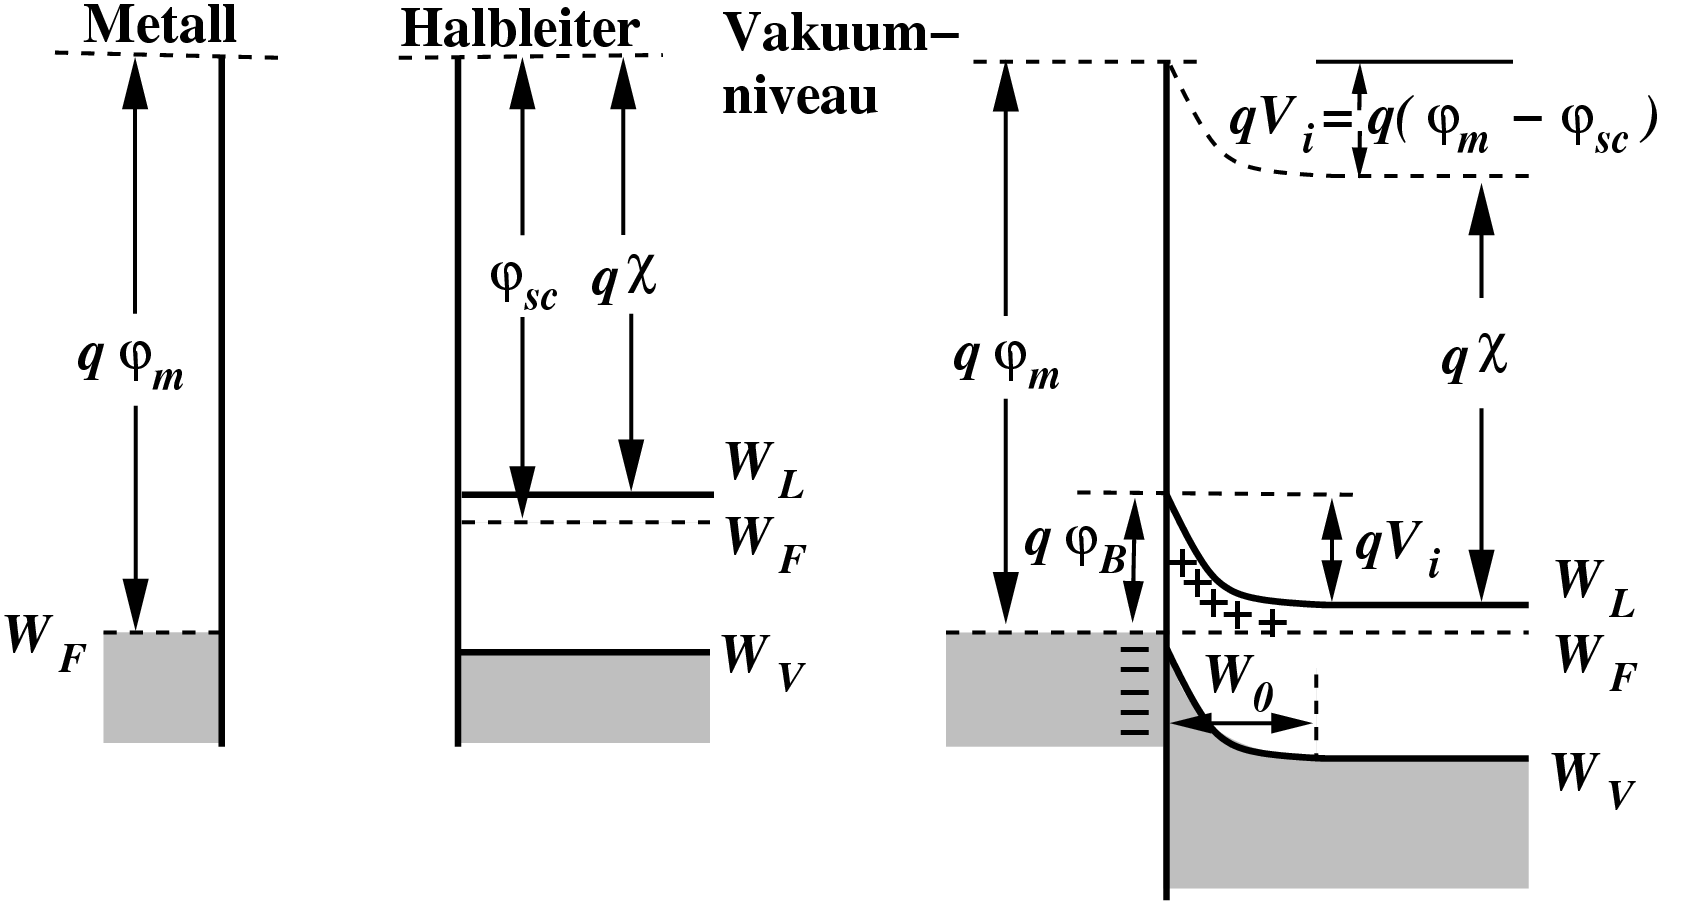
\includegraphics[width=0.75\textwidth]{fig/baenderSchottky}
    \caption{Baenderdiagramm vor und nach dem zusammenlegen von Halbleiter und Metall}
    \label{fig:baenderSchottky}
\end{figure}

\subsection{Tunneldiode \todo{4x}}\label{k5:tunnelDiode}
Die Tunneldiode hat ein hochdotiertes n-leitendes Germanium-Plättchen in das eine ebenfalls hochdotierte Indium-Pille einlegiert ist.
Wegen der hohen Dotierung wirkt die Sperrschicht nicht. Die Sperrschicht wird durch die Elektronen mit hoher Geschwindigkeit durchtunnelt. Die Elektronen durchfliegen nahezu mit Lichtgeschwindigkeit diesen Tunnel. Schon bei einer kleinen Durchlassspannung fließt ein Strom, obwohl die Sperrschicht noch nicht abgebaut ist.

In \Cref{fig:tunneldiode0V} sieht man wie die hohe dotierung zu einer Verschiebung des Fermi-Niveaus ins Leitungs- bzw. Valenzband f\"uhrt.
    \begin{figure}[H]
        \centering
        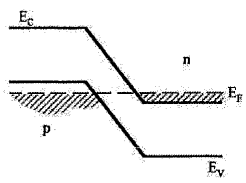
\includegraphics[width=0.4\textwidth]{fig/tunneldiode0V}
        \caption{Banddiagramm der Tunneldiode ohne externe Spannung}
        \label{fig:tunneldiode0V}
    \end{figure}
In \Cref{fig:tunneldiodeFlusspolung} werden schon durch eine kleine Spannung die Energieb\"ander der n-Seite
so weit nach oben verschoben, dass die Elektronen des Leitungsbandes in die leeren Zust\"ande am oberen Ende des Valenzbandes tunneln k\"onnen. Wo das maximum dieses Stroms liegt ist von der Fl\"ache der pn-Zone abh\"angig (typisch $\approx 100mV$).\\
Wird die Spannung gr\"oßer, steht den Leitungselektronen der n-Seite das verbotene Band der p-Seite gegen\"uber.
In diesem Abschnitt hat die Diode einen negativen differentiellen Widerstand, der zur Schwingungserzeugung
und Verst\"arkung genutz werden kann.\\
Bei noch gr\"oßerer Spannung setzt dann der normale Diffusionsstrom ein.
    \begin{figure}[H]
        \centering
        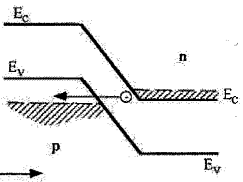
\includegraphics[width=0.4\textwidth]{fig/tunneldiodeFlusspolung}
        \caption{Banddiagramm der Tunneldiode mit Polung in Flussrichtung}
        \label{fig:tunneldiodeFlusspolung}
    \end{figure}
In \Cref{fig:tunneldiodeSperrpolung} ist die Tunneldiode in Sperrrichtung gepolt abgebildet.
    \begin{figure}[H]
        \centering
        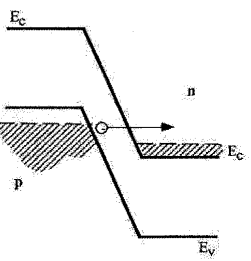
\includegraphics[width=0.4\textwidth]{fig/tunneldiodeSperrpolung}
        \caption{Banddiagramm der Tunneldiode mit Polung in Sperrrichtung}
        \label{fig:tunneldiodeSperrpolung}
    \end{figure}
    
    \subsubsection{Banddiagramm ohne externe Spannung}
    Siehe \Cref{fig:tunneldiode0V}
    \subsubsection{was passiert, wenn 25mV in Flussrichtung angelegt werden?}
    Es wird getunnelt (Siehe \Cref{fig:tunneldiodeFlusspolung})
    \subsubsection{im Banddiagramm Konstellation aufzeichnen, wo Maximum und Minimum in Kennlinie auftreten}
    Maximum in \Cref{fig:tunneldiodeFlusspolung}. F\"ur minimum die B\"ander des n-Bereichs so weit rauf zeichnen
    dass es dem Verbotenen Bereich des p-Bereichs gegen\"ubersteht.
    \subsubsection{Dicke Raumladungszone Dotierung}
    ???
    \subsubsection{Wie groß ist die Bandlücke in Volt}
    ???
    \subsubsection{Kennlinie der Tunneldiode}
    Siehe \Cref{fig:tunneldiodeKennlinie}.\\
    Merkmale:
    \begin{itemize}
        \item Keine Sperrfunktion
        \item Auch bei kleinen Spannungen wird durchgeschalten
        \item Es gibt einen Bereich mit negativem Widerstand
    \end{itemize}
    \begin{figure}[h]
        \centering
        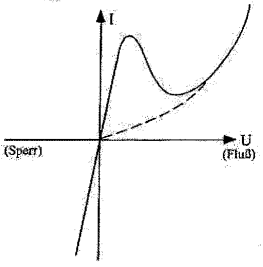
\includegraphics[width=0.75\textwidth]{fig/tunneldiode}
        \caption{Kennlinie der Tunnel-Diode}
        \label{fig:tunneldiodeKennlinie}
    \end{figure}
    
    \subsubsection{Kennlinie einer normalen Diode}
    Siehe \Cref{k5:diode}.

\subsection{Backward-Diode \todo{0x}}\label{k5:backward}
Die Backward-Diode ist eine Tunneldiode mit schw\"acherer Dotierung. Das Strommaximum und der fallende Ast
auf der Flu{\ss}seite verschwinden, es bleibt nur der steile Stromanstieg in Sperrrichtung \"ubrig.
Die starke Nichtlinearit\"at wird zur Gleichrichtung schwacher Signale und zur Mischung im Mikrowellenbereich
genutzt.

\subsection{Heterostrukturen \todo{0x}}\label{k5:heterostrukturen}

%--------------------------------------------------------------------------------
%--------------------------------------------------------------------------------
%--------------------------------------------------------------------------------

\section{Transistoren - Kapitel 6}\label{k6:transistoren}
%--------------------------------------------------------------------------------
%--------------------------------------------------------------------------------
%--------------------------------------------------------------------------------

Ein Transistor besteht prinzipiell aus zwei PN-Übergängen, also zwei Dioden. 
Der Emitter-Basis Übergang ist üblicherweise (für einen Verstärkungsbetrieb) in Flussrichtung geschalten und der Basis-Kollektor Übergang in Sperrichtung. 

\subsection{Funktion von Bipolartransistoren \todo{1x}}\label{k6:bipolar}
Die folgenden Beschreibungen gelten immer für den npn Transistor (\autoref{fig:transistor-npn} wenn nicht anders erwähnt.    
    \begin{figure}
        \centering
        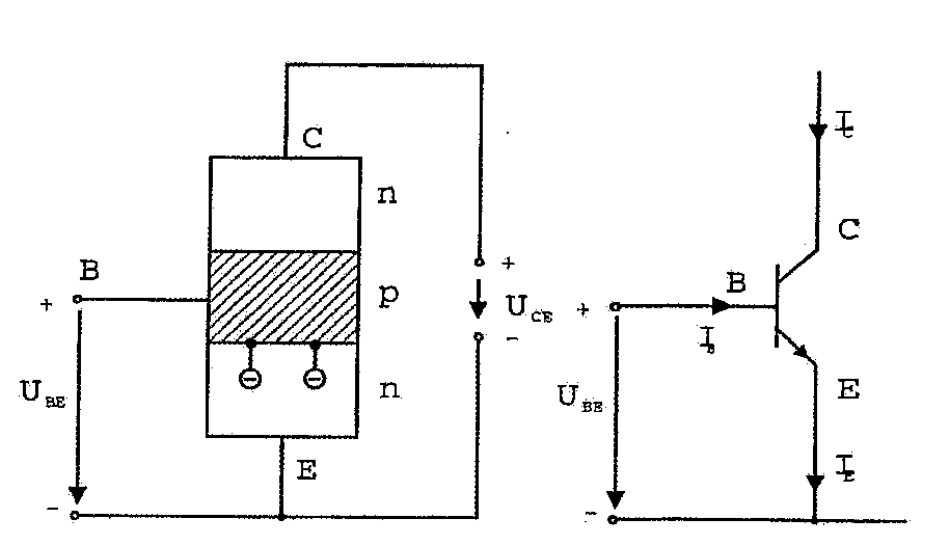
\includegraphics[width=0.66\textwidth]{fig/npn-transistor}
        \caption{NPN Bipolar Transistor}
        \label{fig:transistor-npn}
    \end{figure}
    
    \begin{figure}
        \centering
        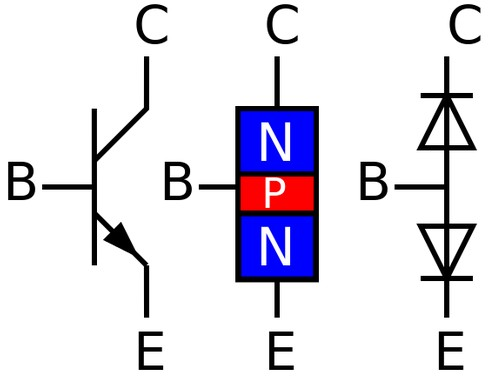
\includegraphics[width=0.33\textwidth]{fig/transistor-npn-diode.jpg}
        \caption{NPN Transistor und sein Diodenersatzschaltbild.}
        \label{fig:transistor-npn-diode}
    \end{figure}
    
    \begin{figure}
        \centering
        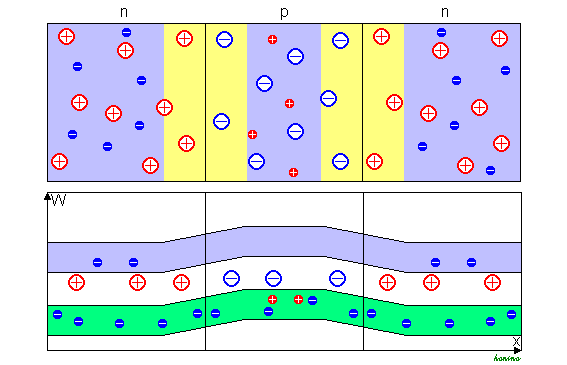
\includegraphics[width=0.33\textwidth]{fig/npn-bipolartransistor-band1.PNG}\hfill
        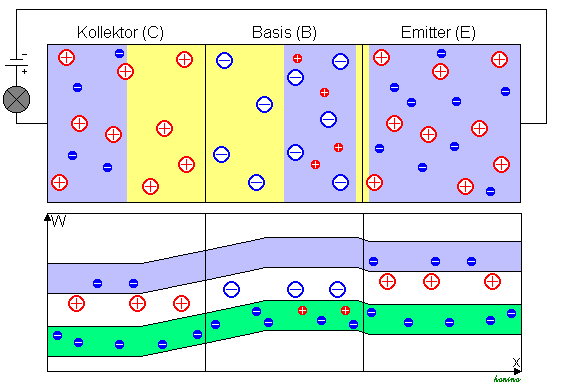
\includegraphics[width=0.33\textwidth]{fig/npn-bipolartransistor-band2.PNG}\hfill
        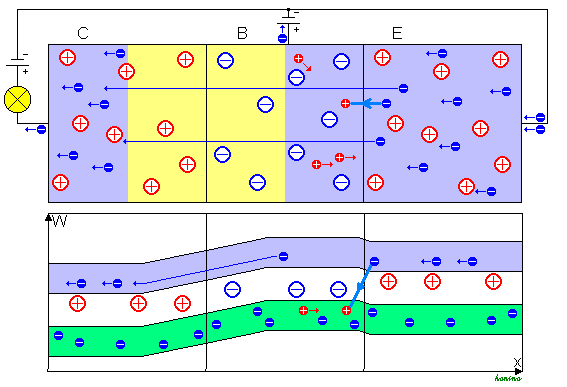
\includegraphics[width=0.33\textwidth]{fig/npn-bipolartransistor-band3.PNG}
        \caption{\textbf{Links:} Kristallaufbau und Bändermodell eines Bipolartransistors. \textbf{Mitte:} Selbiges bei angelegter Kollektor-Emitter Spannung. \textbf{Rechts:} Zusätzlich mit angelegter Basis-Emitter Spannung.}
        \label{fig:npnTransistor}
    \end{figure}
    
    \subsubsection{Physikalischer Aufbau}
    Ein Bipolartransistor besteht aus drei dünnen Halbleiterschichten, die übereinander gelegt sind. Die mittlere Schicht ist im Vergleich zu den zwei äußeren Schichten sehr dünn.
    
    \subsubsection{Funktionionsweise}
    Durch einen kleinen elektrischen Strom $I_B$ an der Basis wird ein größerer Strom $I_C$ zwischen Kollektor und Emitter gesteuert. 
   
   \begin{enumerate}
    \item \emph{Aktive Kollektor-Emitter Spannug $U_{CE} > 0$:} Wird nur eine Spannung zwischen Kollektor und Emitter angelegt ($U_{CE} > 0$), entspricht das Schaltungstechnisch einfach zwei entgegengesetzten Dioden, von denen eine immer gesperrt ist (Für npn ist das die Basis Kollektor Diode). 
    Die angelegte Spannung verringert zwar die Basis-Emitter Sperrschicht, die Basis-Kollektor Sperrschicht (auch Raumladungszone) vergrößert sich aber gleichzeitig.  
    
    \item \emph{Zuschaltung von $U_{BE} > 0.7$:} Wird nun zusätzlich eine Basis Emitter Spannung von mehr als 0.7V angelegt, dann werden Elektronen aus dem Emitter in die Basis injiziert. Diese Elektronen rekombinieren prinizpiell mit den Löchern in der Basis. Da die Basis aber sehr, sehr klein ist, diffundieren mehr als 99\% der Elektronen in die Basis-Kollektor Sperrschicht. Da bereits eine Spannung $U_{CE} > 0$ anliegt, wandern die Elektronen durch die Potentialdifferenz gleich weiter aus dem Kollektor hinaus. Dieser vom Emitter zum Kollektor fließende Storm ist dann $I_C$.
    
    
    \item \emph{Durchlass (anders formuliert, sonst wie 2:} Wird eine Spannung $U_{BE} > 0.7V$ zwischen Basis und Emitter angelegt, dann kann das elektrische Feld der Raumladungszone von Elektronen überwunden werden.
    Dabei gelangen die Elektronen von der n-Schicht des Emitters in die p-Schicht der Basis und können von dort aus der Basis hinaus fließen, da sie von der positiven Seite der Spannungsquelle (die auch $U_{BE}$ erzeugt) angezogen werden.
    Da aber die p-Schicht so klein ist, können nicht alle Elektronen über die Basis abfließen sondern wandern weiter in die obere Grenzschicht.
    
    Die vom Emitter in die Basis injizierten Elektronen werden von der Basis-Collector Raumladungszone abgesaugt und fließen \textit{nicht} über den Basisanschluss. 
   \end{enumerate} 
    
    
    \subsubsection{Skizze}
    
    \begin{figure}
        \centering
        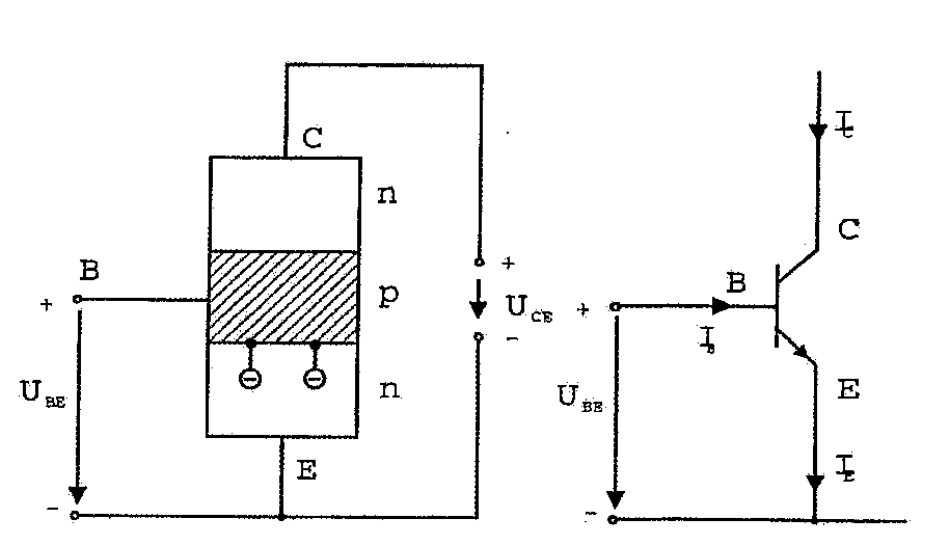
\includegraphics[width=0.66\textwidth]{fig/npn-transistor.jpg}
        \caption{Schematischer Aufbau und Schaltsymbol des npn-Transistors}
        \label{fig:npnTransistor}
    \end{figure}
    
    \begin{figure}
        \centering
        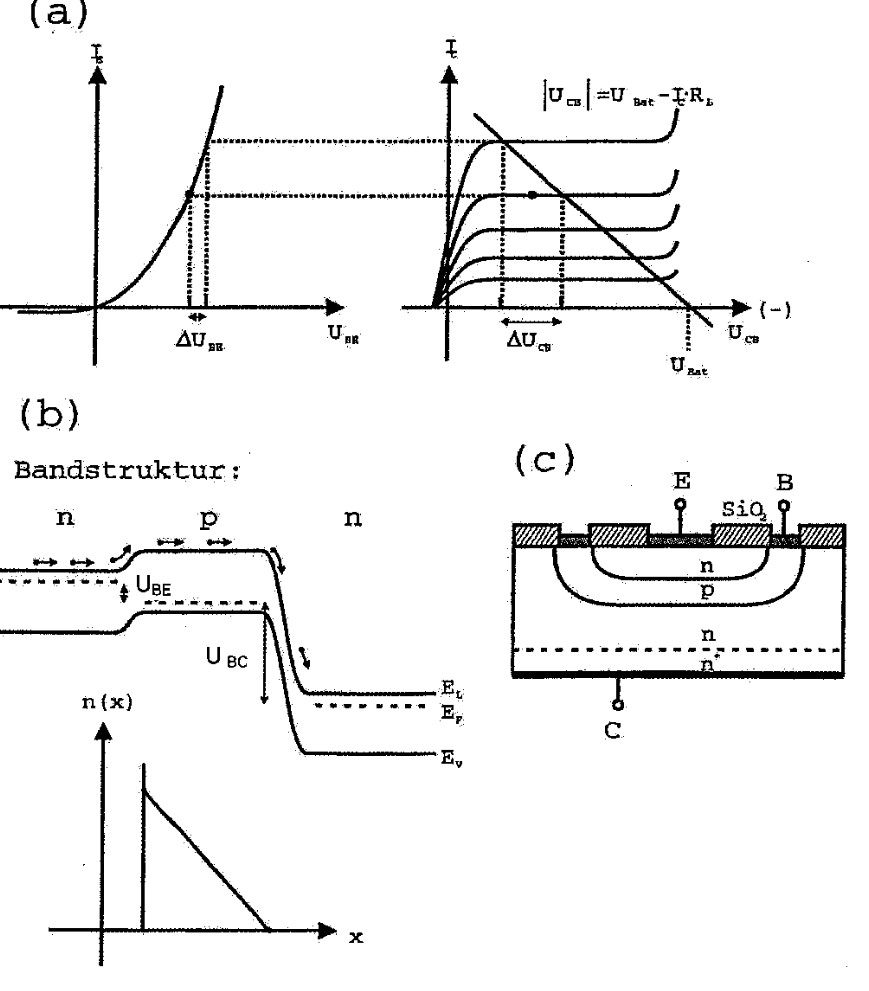
\includegraphics[width=0.66\textwidth]{fig/npn-transistor-kennlinien.jpg}
        \caption{Transistor - eine Hintereinanderschaltung zweier Dioden. Steile EB-Durchlasskennlinie steuer hochohmige EC-Diode. Weiters sind die Bandstruktur im Ort, der schematische AUfbau und das Diffusionsdreieck dargestellt.}
        \label{fig:npnTransistorKennlinie}
    \end{figure}
    
    \subsubsection{Warum wird er als Verst\"arker eingesetzt?}
     
    
\subsection{MOS-Struktur und Inversion \todo{2x}}\label{k6:mosInversion}

    \subsubsection{Wann spricht man von Inversion}
    Von MOS-Inversion spricht man, wenn sich die Ladungsträgerdichten in einem Halbleiter lokal ändern und er seine Eigenschaften aus dem Grundzustand "verliert".
    
    \emph{Exakte Definition:} Die Inversion ist dann erreicht, wenn die Zahl der Elektronen an der Oberfläche gleich groß ist, wie die Zahl der Löcher im Volumen des Halbleiters. Diese Situation ist dann gegeben, wenn die Bandverbiegung $\Phi_S = 2\Phi_F$ ist.Die äußere Spannung die dazu notwendig ist, wird dementsprechend auch Schwellwertspannung (Thresholdvoltage) genannt. \autoref{fig:mos-energie} zeigt die Energieniveaus.
    
    \begin{figure}
        \centering
        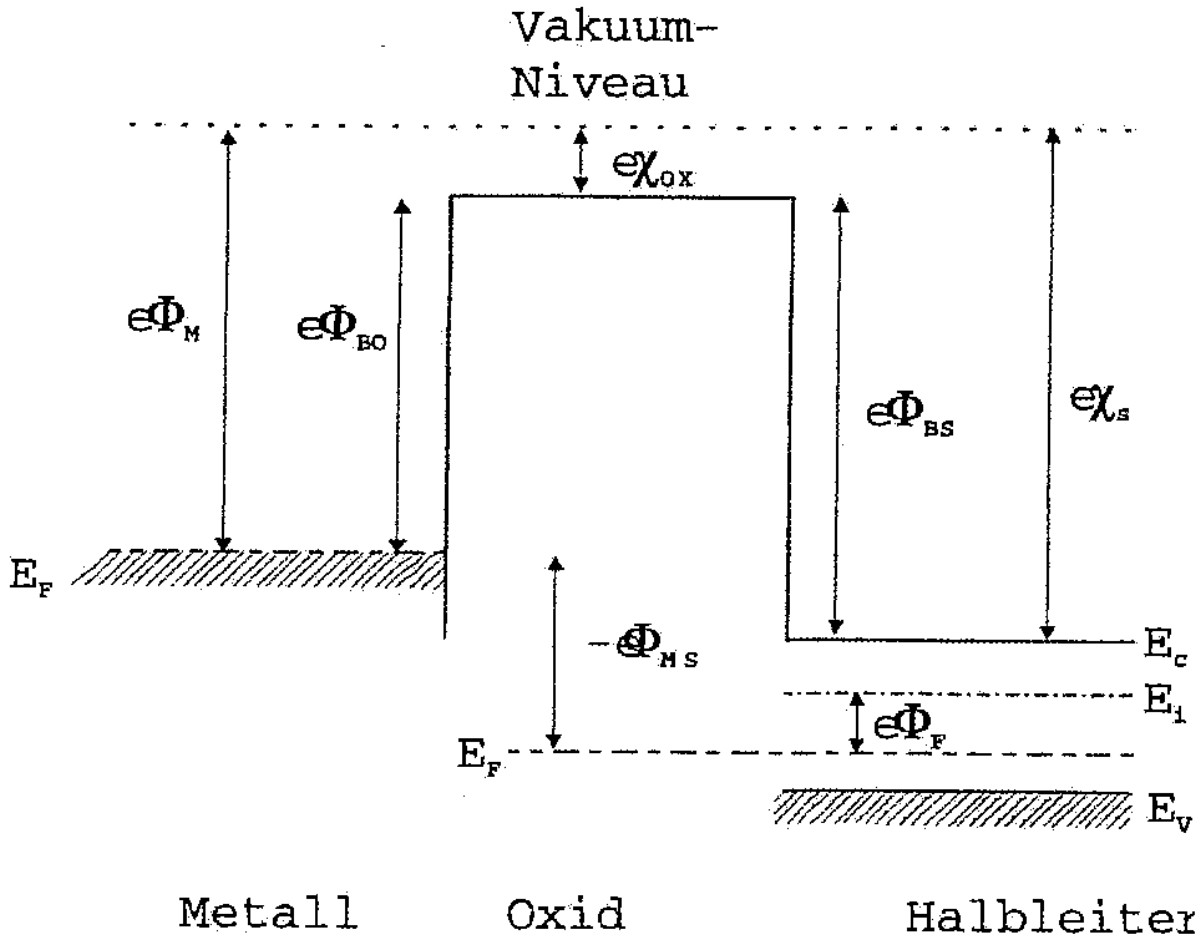
\includegraphics[width=0.66\textwidth]{fig/mos-energie.jpg}
        \caption{Energetische Verhältnisse in einer Metall-Oxid Halbleiter-Struktur unter Flachband-Bedingungen. }
        \label{fig:my_label}
    \end{figure}
    
    \emph{Beispiel P-MOS: \autoref{fig:mos-inversion2}}
    \begin{enumerate}
        \item Der Halbleiter ist p-dotiert, d.h. es gibt mehr Löcher als Elektronen.
        \item Am Gate wird eine negative Spannung angelegt, d.h. die Dichte an Löchern erhöht sich dort und es entsteht ein starker Potentialgradient zum Halbleiter.
        \item Alle freien Elektronen des Halbleiters wandern in Richtung des Gates um den Gradient wieder auszugleichen.
        \item Entlang des Gates entsteht eine Zone mit mehr freien Elektronen als Löchern. Lokal betrachtet verhält sich der Halbleiter hier also eher wie ein n-dotierter Halbleiter, nicht wie ein p-dotierter. Daher der Name \textbf{MOS-Inversion}.
    \end{enumerate}
    
    \begin{figure}[H]
        \centering
        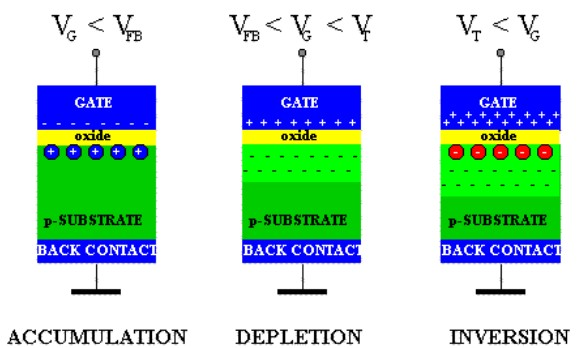
\includegraphics[width=0.33\textwidth]{fig/mos-inversion.jpg}
        \caption{Ganz rechts: Die Inversion in einem MOS mit p-Substrat.}
        \label{fig:mos-inversion2}
    \end{figure}
    
    \subsubsection{Leitungsband, Valenzband, Ef aufzeichnen}

\subsection{Diffusions-Dreieck beim Transistor \todo{0x}}\label{k6:diffusionsdreieck}

\autoref{fig:npnTransistorKennlinie}
    \subsubsection{Warum fast linear?} exponential-Funktion im Ursprung ann\"ahernd linear
    \subsubsection{Was w\"are wenn die Basisl\"ange gr\"o{\ss}er als die Diffusionsl\"ange w\"are?} Man h\"atte die Wirkung von 2 Dioden und keinen Transistoreffekt mehr.

\subsection{Feldeffekt-Transistor \todo{0x}}\label{k6:fet}


\subsection{MOS-FET \todo{0x}}\label{k6:mosfet}

Bipolartransistor kann man sich als 2 Schleusen vorstellen, wobei eine kleine Schleuse über einen Hebel die größere Steuert. 
MOS-FET kann man sich als Wasserschlauch vorstellen, bei dem man von außen drauf treten kann um den Fluss zu regulieren.
Daran kann man relativ schnell erkennen, dass ein MOS-FET a.) weniger Strom braucht und b.) schneller schaltet als ein Bipolartransistor. 

Die wichtigsten Begriffe in einem MOS-System sind Akkumulation, Verarmung und Inversion.
Diese Breiche sind quantitativ über die Flachbandspannung $V_FB$ (Die externe Spannung, zur der es im Halbleiter keine Bandverschiebung gibt) definiert. 
Hier kurz für p-dotiertes Silizium:
\begin{enumerate}
    \item Akkumulationsbereich ($V_G \ll V_{FB}$): Hauptsächlich Majoritätsladungsträger (Löcher) unter der Gate Elektrode (\autoref{fig:mos-akkumulation})
    \item Verarumungsbereich ($V_G > V_{FB}$): WEniger Majoritätsladungsträger (Löcher) unter der Gate-Elektrode als normal (\autoref{fig:mos-verarmung}) 
    \item Inversionbereich ($V_G \gg V_{FB}$): Es sammeln sich Minoritätsladungsträger (Elektronen) unter dem Gate. (\autoref{fig:mos-inversion}) 
\end{enumerate}

    \begin{figure}[H]
        \centering
        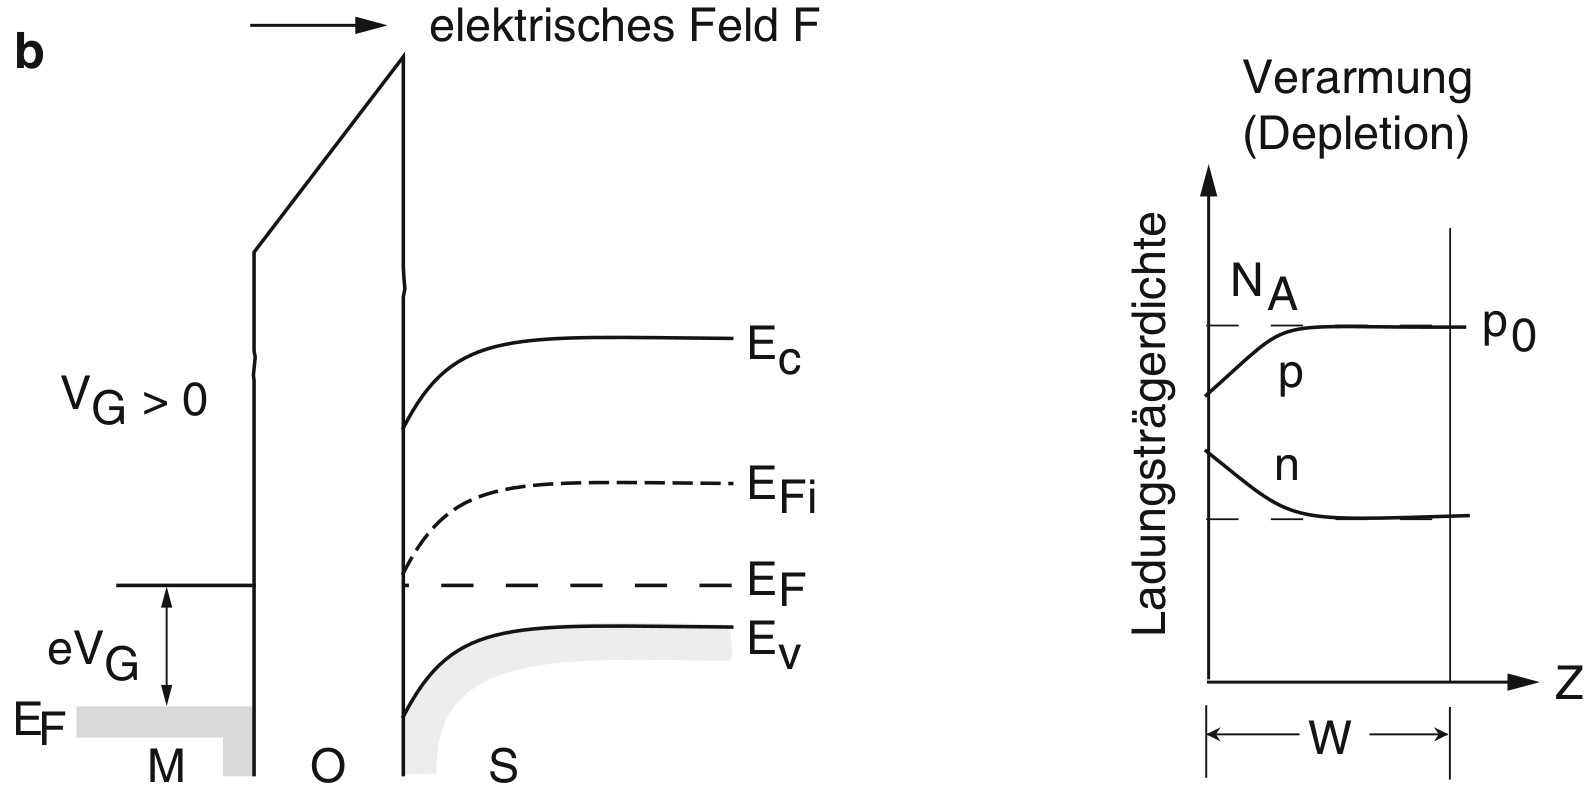
\includegraphics[width=0.66\textwidth]{fig/mos-verarmung}
        \caption{MOS Band-Diagramm und Ladungsträgerdichte für Verarmung.}
        \label{fig:mos-verarmung}
    \end{figure}
    \begin{figure}[H]
        \centering
        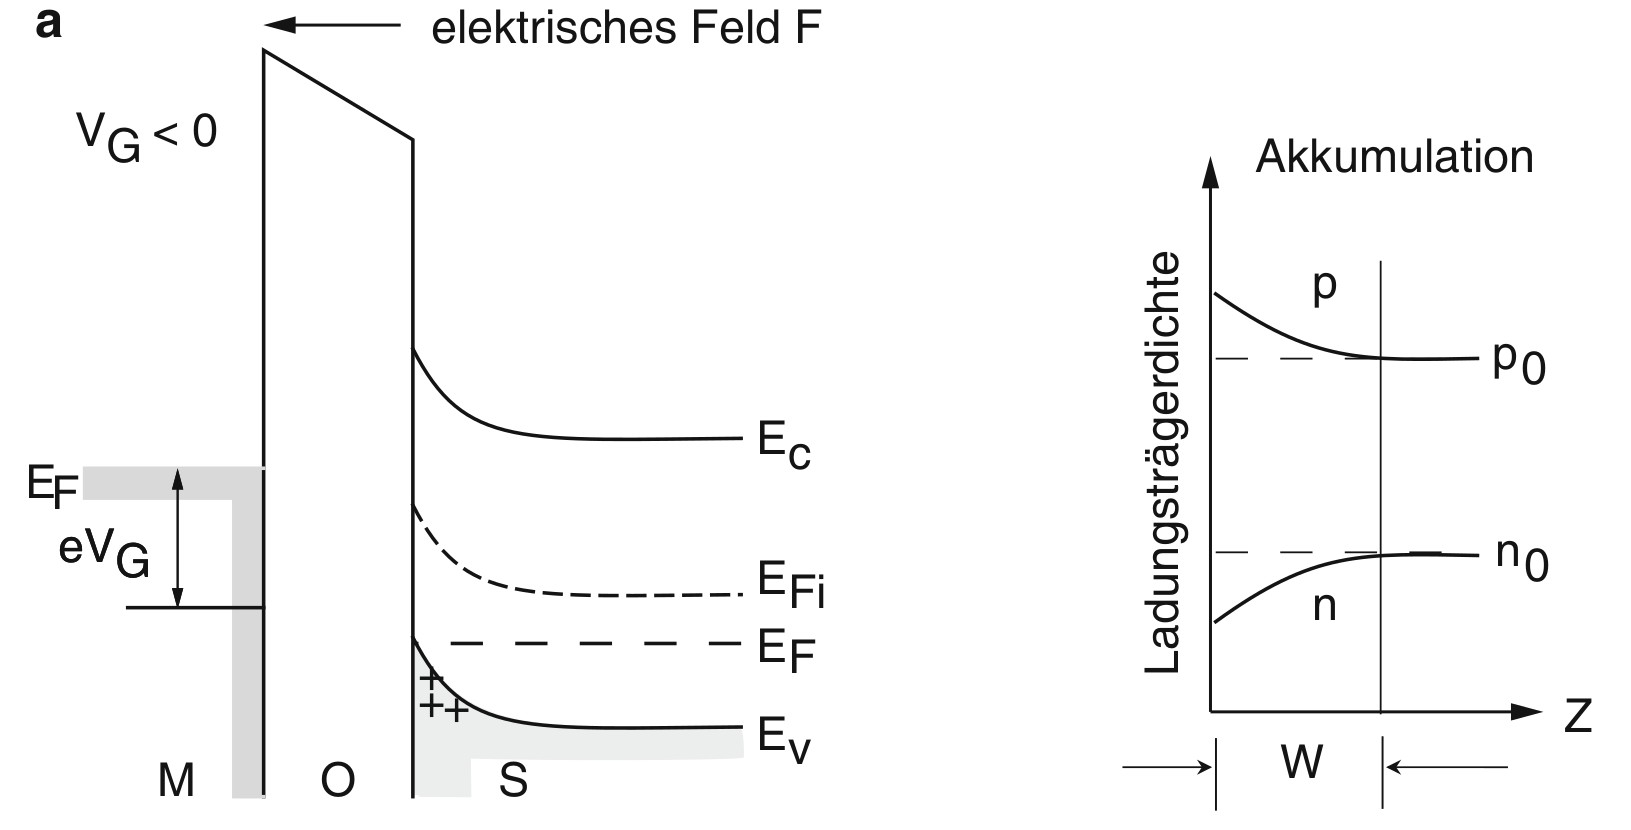
\includegraphics[width=0.66\textwidth]{fig/mos-akkumulation}
        \caption{MOS Band-Diagramm und Ladungsträgerdichte für Akkumulation.}
        \label{fig:mos-akkumulation}
    \end{figure}
    \begin{figure}[H]
        \centering
        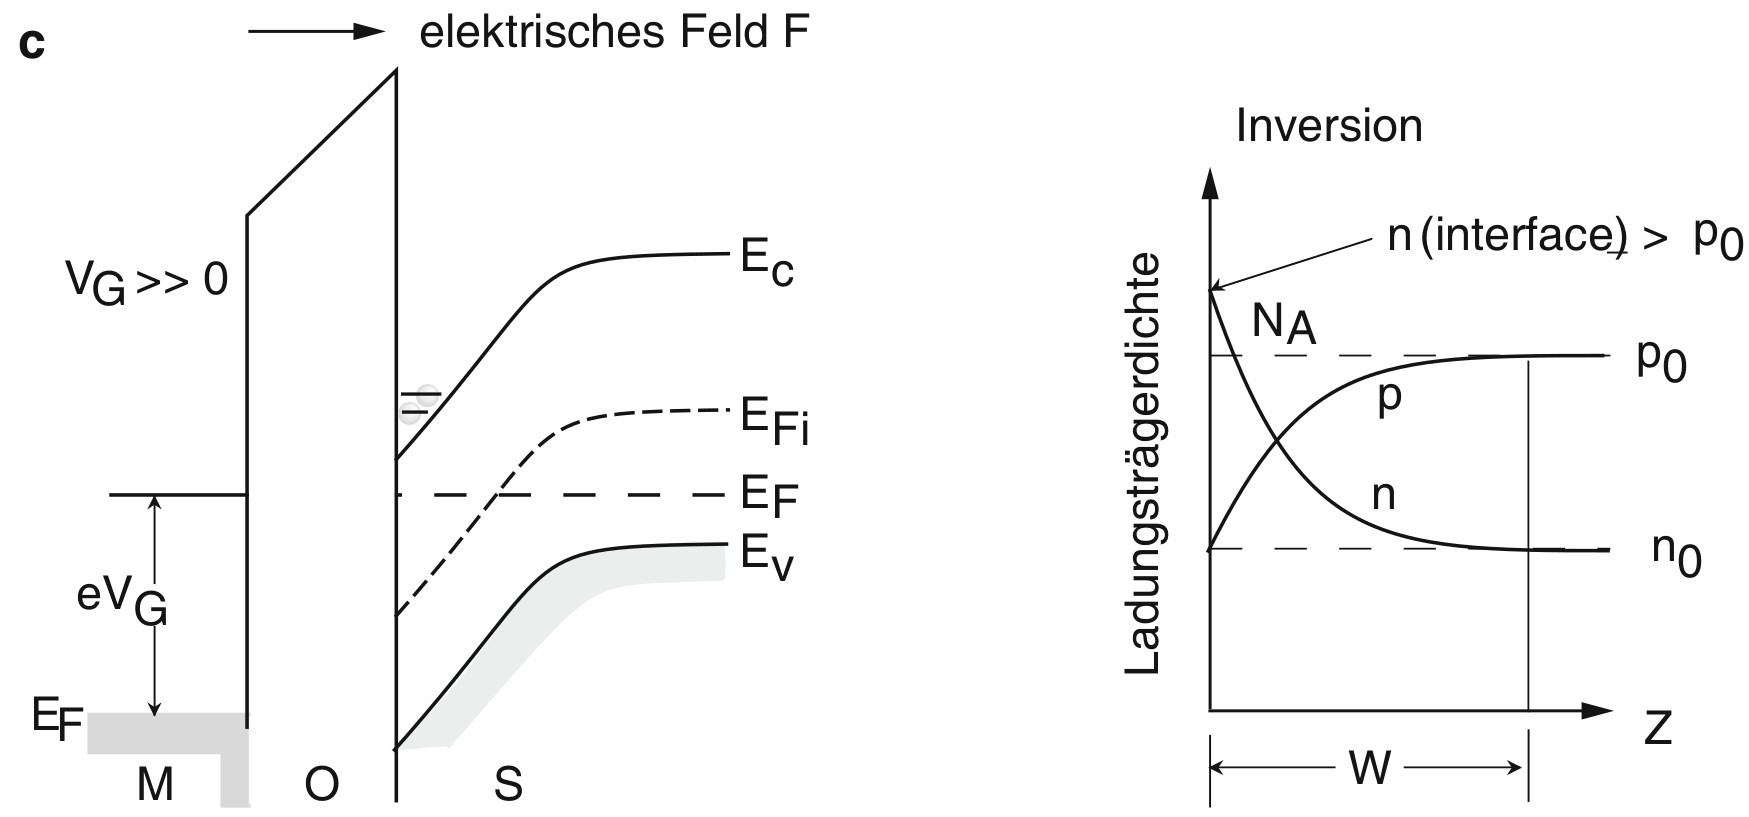
\includegraphics[width=0.66\textwidth]{fig/mosfet-inversion}
        \caption{MOS Band-Diagramm und Ladungsträgerdichte für Inversion.}
        \label{fig:mos-inversion}
    \end{figure}

    \subsubsection{Aufbau}
    Siehe \autoref{fig:mos-aufbau}, \autoref{fig:mos-aufbau2}.
    \begin{figure}[H]
        \centering
        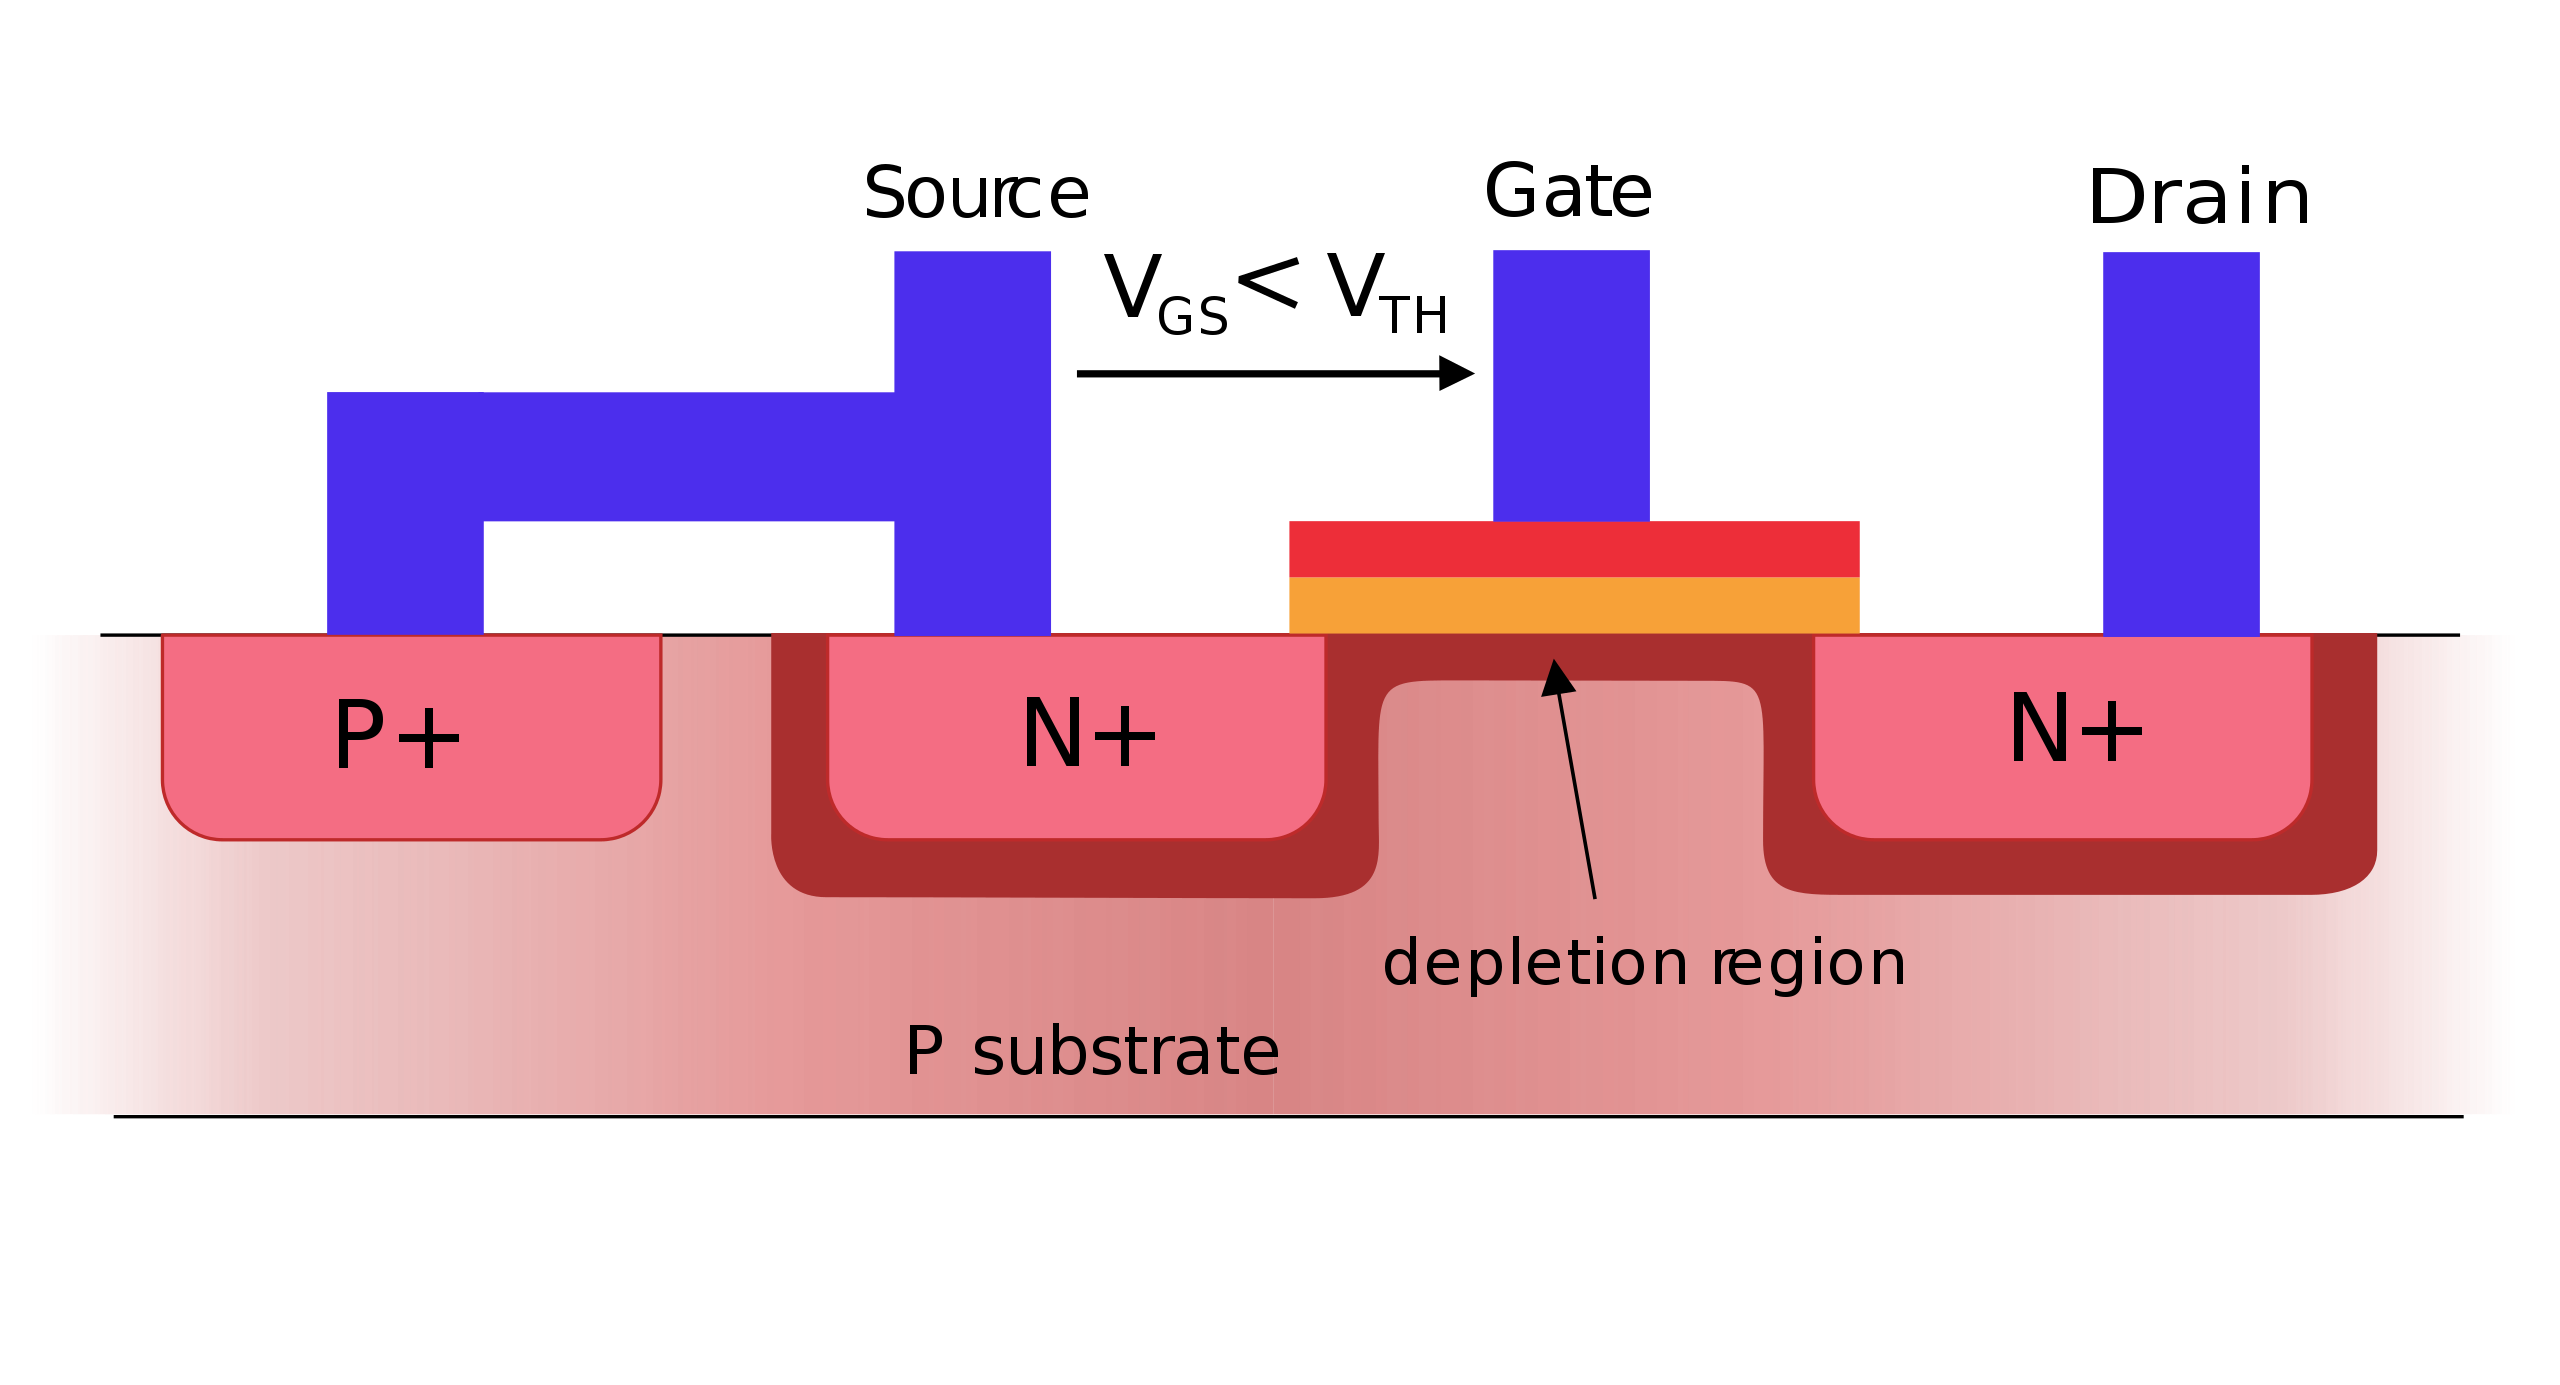
\includegraphics[width=0.66\textwidth]{fig/mos-aufbau.png}
        \caption{A cross-section through an nMOSFET when the gate voltage VGS is below the threshold for making a conductive channel; there is little or no conduction between the terminals drain and source; the switch is off. When the gate is more positive, it attracts electrons, inducing an n-type conductive channel in the substrate below the oxide, which allows electrons to flow between the n-doped terminals; the switch is on.}
        \label{fig:mos-aufbau}
    \end{figure}
    
    \begin{figure}[H]
        \centering
        \includegraphics[width=0.66\textwidth]{fig/mos-aufbau2}
        \caption{Nochmal der Aufbau eines MOSFETs.}
        \label{fig:mos-aufbau2}
    \end{figure}
    
    \subsubsection{Flachband und Inversion}
    Wird eine Spannung am Gate angelegt (für p-MOS), dann werden die Löcher in das innere des Halbleiters verschoben (Also vom Gate weg). Es entsteht also eine \textit{Verarmungszone}, in der Elektronen dominieren. Diese Verarmungszone kann man wie eine Raumladungszone betrachten - es gibt keine leitende Verbindung zwischen Source und Drain.
    
    Erreicht die Gatespannung aber den Schwellwert $U_T$ (Thresholdspannung), dann bildet sich an der Halbleiteroberfläche eine sogenannte \textit{Inversionsschicht} aus, in der Elektronenleitung auftritt. Damit besteht eine leitende Verbindung zwischen Source und Drain, der sogenannte \textit{Kanal}. 
    
    Im \textit{Flachbandfall} ist die Löcherdichte an der Grenzfläche exakt gleich wie im Inneren des Substrates. Wird die Bandverbiegung so groß, dass das Leitungsband an der Grenzfläche dem Ferminiveau nahe kommt, treten an der Grenzfläche Elektronen auf. 
    
    
    \subsubsection{Bandstruktur}
    
    \begin{figure}
        \centering
        \includegraphics[width=0.66\textwidth]{fig/mos-bänder2.jpg}
        \caption{Bandschema des MOSFET normal zur Oberfläche für verschiedene Gatespannungen. 
        Links ist immer das Oxid eingezeichnet, das Band entfernt sich dann weg vom Oxid. Akkumulation, Verarmung, FLachbandfall, Inversion.}
        \label{fig:mos-bänder2}
    \end{figure}
    
    
    \begin{figure}
        \centering
        \includegraphics[width=0.66\textwidth]{fig/mos-bänder1.jpg}
        \caption{(a) Aufbau einer MOS-Struktur. (b) Austrittsarbeiten, Nadlücken, Fermi-Niveaus etc. in einem Metall, einem Oxi und einem Halbleiter}
        \label{fig:mos-bänder1}
    \end{figure}
    
    \begin{enumerate}
        \item $\Phi_S$: Austrittsarbeit (Abstand vom Fermi-Niveau zum Vakuum) im Halbleiter
        \item $\Xi$ Energieabstand zwischen Leitungsband un dVakuum
        \item $\Phi_B^n = \frac{kT}{e}ln(\frac{N_D}{n_i})$: Abstand zwischen Fermi-Niveau und Leitungsband im n-Typ-Halbleiter
        \item $\Psi(z) = \Phi(z) - \Phi_B$ Bandverbiegung
        \item $V_{FB}$: Flachbandspannung: Extern angelegte Spannung, bei der es keine Bandverbiegungen im Halbleiter gibt. 
        \item $\omega = \sqrt{\frac{2*\Psi_S \epsilon_S}{eN_A}}$: Breite der Verarmungszone (depletion zone) im Halbleiter, hier für das p-Typ-Silizium
    \end{enumerate}
    
    \begin{figure}
        \centering
        \includegraphics[width=0.66\textwidth]{fig/mos-leitungsband.jpg}
        \caption{Leitungsbandprofil der fertigen MOS-Struktur.}
        \label{fig:mos-bänder}
    \end{figure}
    

\subsection{MES-FET \todo{0x}}\label{k6:mesfet}

\subsection{Early-Effekt \todo{0x}}\label{k6:early}
Eine kleine Abhängigkeit des Kollektorstromes von $U_{CB}$ wird durch den sogenannten
Early-Effekt verursacht. Eine höhere Sperrspannung $U_{CB}$ bewirkt eine wachsende RLZ
zwischen C und B. Der rechte Rand der neutralen Basiszone wandert somit etwas nach
links, der Effektivwert von W wird kleiner, das Diffusionsdreieck steiler und $I_C$ größer.
Bei sehr großem $U_{CB}$ frisst die RLZ die gesamte Basis auf: Dieser Punch-through-Effekt
stellt eine Grenze für $U_{CB}$ dar.

\begin{enumerate}
    \item \emph{Ursache:} Wird die Kollektor-Emitter Spannung erhöht, dann vergrößert sich die Raumladungszone des Kollektor-Basis Übergangs und die Weite der Basis verringert sich.
    \item \emph{Auswirkung:} Der Transistor ist keine ideale Stromquelle, da der Kollektorstrom von der Kollektor-Emitter Spannung $U_{CE}$ abhängt.
    \item \emph{Größenordnung:} Liegt bei Transistoren betragsmäßig zwischen 15V und 150V. 
\end{enumerate}

Eine verkleinerte Basis hat zur folge, dass Elektronen mit einer geringeren Wahrscheinlichkeit in der Basis rekombinieren.
Daraus folgend müssen mehr Elektronen über den Kollektor fließen, der Strom erhöht sich in einer nicht-linearen Art und Weise. 

    \begin{figure}
        \centering
        \includegraphics[width=0.66\textwidth]{fig/transistor-early-effect.png}
        \caption{Early-Spannung ist der Punkt ganz links}
        \label{fig:npnTransistorKennlinie}
    \end{figure}


\subsection{JFET \todo{0x}}\label{k6:jfet}

    \begin{figure}[H]
        \centering
        \includegraphics[width=0.66\textwidth]{fig/jfet-aufbau.jpg}
        \caption{Aufbau eines Sperrschichtfeldeffekt Transistors (JFET - \textbf{J}unction \textbf{F}ield \textbf{E}ffect \textbf{T}ransistor)}
        \label{fig:jfet-aufbau}
    \end{figure}

In \autoref{fig:jfet-aufbau} ist der Aufbau eines n-Kanal Sperrschicht-Feld Effekt Transistors zu sehen. 

Im Transistor befindet sich ein n-leitender Kanal, durch den Elektronen von der Source Elektrode S zur Drain Elektrode D fließen können, wenn $U_{DS} > 0$ ist (Drain-Source Spannung).

Die steuernde Gate Elektrode G ist leitend mit einer p-dotierten Zone verbunden, die durch eine Sperrschicht vom Kanal getrennt ist. 
Für $U_{GS} > 0$ ist dieser pn-Übergang in Sperrichtung gepolt.

\subsubsection{JFET vs MOSFET}
JFET und MOSFET haben nahezu identische Eigenschaften. Abgesehen von den verschiedenen Herstellungsverfahren ist als Unterschied hervorzuheben, dass für den JFET nu rjene Polarität von $U_{GS} $ verwendet werden darf, für die das Gate-Gebiet gegen den Kanal in Sperrrichtung gepolt ist. 

\subsubsection{FET vs Bipolar-Transistor}

\textbf{Vorteile FET}
\begin{enumerate}
    \item Sehr kleiner Gatestrom bei Gleichspannung (MOSFET $I_G < ipA$)
    \item Im Schalterbetrieb müssen keine Speicherladungen abgeführt werden. 
    \item Die Schwellspannung kann in weiten Grenzen bei der Herstellung eingestellt werden.
    \item Leichte Integrierbarkeit des MOSFET (nicht für JFET). Weit weniger verschiedene Diffusionsprozesse und photolithographische Prozesse bei der Herstellung nötig und der Platzbedarf ist geringer.
    \item Geringes Rauschen
    \item Keine Offset Spannung bei Zerhacker Anwendungen, weil sich im eingeschalteten Zustand der Kanal wie ein ohmscher Widerstand verhält, d.h. $I_D=0$ für $U_{DS} = 0$
    \item Unempfindlicher gegenüber Strahlungsschäden
    \item Schwächere Temperaturabhängigkeit. Im Bipolar ist die Minoritätendichte wesentlich, die proportional zu $n_i^2$ und daher exponentiell mit der Temperatur steigt. Die im FET ausgenützte Leitfähigkeit der Majoritäten hingegen ändert sich nur über die Beweglichkeit $\mu$ in der Temperatur. Da die Beweglichkeit mit der steigenenden Temperatur sinkt, sinkt acuh $I_D$ mit der Temperatur. Der FET ist demnach thermisch selbststabilisierend.
\end{enumerate}

\textbf{Vorteile Bipolartransistor}
\begin{enumerate}
    \item Sehr große Steilheit. Ermöglicht große Kleinsignalverstärkung. 
    \item Hohe Grenzfrequenz. 
    \item Die Steuerkennline $I_C(U_{BE}$ des Bipolartransistors ist kleineren Exemplarstreuungen unterworfen als jene des FET. 
\end{enumerate}

%--------------------------------------------------------------------------------
%--------------------------------------------------------------------------------
%--------------------------------------------------------------------------------
\newpage
\section{Formelsammlung}

Impuls ist Abhängig von der Wellenzahl $k$:
\begin{equation}
    p = \hbar \cdot k
\end{equation}

\hrule
\vspace{0.5cm}
\textbf{Compton Effekt} durch elastischen Stoß:

\begin{enumerate}
    \item $E_e$ ... kinetische Energie
    \item $\vec{p_e}$ ... Impuls des Compton-Elektrons
    \item $\vec{k}$ ... Wellenvektor, zeigt die Ausbreitungsrichtung des Photons
\end{enumerate}

\begin{equation}
    \hbar \omega_0 = \hbar \cdot \omega_{SC} + E_e
\end{equation}

\begin{equation}
    \hbar \vec{k_0} = \hbar \cdot \vec{k_{SC}} + \vec{p_e}
\end{equation}

Länge des Wellenvektors $\vec{k}$, zeigt in die Ausbreitungsrichtung des Photons
\begin{equation}
    |\vec{k}| = \frac{2\pi}{\lambda}
\end{equation}

Impuls einen Photons:
\begin{equation}
    |\hbar \vec{k}| = \frac{h}{\lambda}
\end{equation}

Energie eines Photons:
\begin{equation}
   E = \hbar \omega 
\end{equation}

\hrule
\vspace{0.5cm}

\textbf{Materiewellen} nach De Broglie - die Wellenlänge hängt nur vom Teilchenimpuls ab:
\begin{equation}
    \lambda = \frac{h}{p}
\end{equation}

\hrule
\vspace{0.5cm}

(Kinetische???) Energie ist Abhängig vom Impuls und der Masse:
\begin{equation}
    E = \frac{p^2}{2m}
\end{equation}

Ansatz für eine planare, zeitabhängige Welle:
\begin{equation}
    \varphi(x,t) = A * e^{-i(kx+\omega t)}
\end{equation}

Harmonische Welle, k ist fürs erste ein Faktor, der das Argument des Sinus dimensionslos macht:
\begin{equation}
    \Psi(x,t) = A * sin(x,t) = A \cdot sin(k\cdot x - k \cdot v \cdot t)
\end{equation}

\hrule
\vspace{0.5cm}

\textbf{Dispersionsrelation} $\omega(k)$

Zusammenhang zwischen Zeitlicher Periodizität $v$ und räumlicher Periodizität $\lambda$ durch $\omega(k)$:

\begin{equation}
    \omega = 2\pi v
\end{equation}

\begin{equation}
    k = \frac{2\pi}{\lambda}
\end{equation}
\hrule
\vspace{0.5cm}

\textbf{Dispersionsrelation in der Teilchenphysik} $\omega(k)$

Frequenz steht im Zusammenhang mit der Energie:
\begin{equation}
    \omega = \frac{E}{\hbar}
\end{equation}

Wellenvektor steht im Zusammenhang mit dem Impuls:
\begin{equation}
    k = \frac{p}{\hbar}
\end{equation}

Energie-Impuls Beziehung der Teilchenphysik wird entsprechend als \textit{Dispersionrelation} bezeichnet.

Für freie Elektronen im nicht-relativistischen Fall zum Beispiel:
\begin{equation}
    E = \frac{p^2}{2m}
\end{equation}

\begin{equation}
    \hbar \omega = \frac{k^2\cdot \hbar^2}{2m}
\end{equation}
\begin{equation}
    \omega = \frac{k^2\cdot \hbar}{2m}
\end{equation}

\hrule
\vspace{0.5cm}

\textbf{Schrödingergleichung, kräftefreies Teilchen, eine Dimension, zeitabhängig}

Für ein kräftefreies Teilchen in einer Dimension (also konstante Energie). 

\begin{equation}
-\frac{\hbar}{2m} \frac{\partial^2}{\partial x^2}\Psi(x,t) = i\hbar\frac{\partial}{\partial t} \Psi(x,t)
\end{equation}

\begin{enumerate}
    \item \textit{Klassisches Teilchen:} Geradlinige und gleichförmige Fortbewegung.
    \item \textit{Wellenbild Teilchen:} Einfachste Form ist eine laufende Welle.
    \item Wellen dieser Form sind Lösungen einer linearen Differentialgleichung zweiter Ordnung (der \textit{Bewegungsgleichung})
    \item \textit{Bewegugnsgleichung}: Beschreibt räumliche und zeitliche Entwicklung eines mechanischen Systems vollständig.
    \item Lösung der Bewegungsgleichung ist die Trajektorie, auf der sich das System bewegt. 
\end{enumerate}

\begin{equation}
   \Psi(x,t) = e^{-i(kx + \omega t)}
\end{equation}

\textbf{Drei Bedingungen} die erfüllt sein müssen:

\begin{enumerate}
    \item Energie muss direkt proportional zur Frequenz sein
    \item Impuls muss direkt proportional zur Wellenzahl $k$ sein
    \item Kinetische Energie muss mit dem Impuls zusammenhängen
\end{enumerate}

\begin{equation}
   E = \hbar \cdot \omega 
   \quad\text{und}\quad
   p = \hbar \cdot k 
   \quad\text{und}\quad
   E_{kin} = \frac{p^2}{2m}  
\end{equation}

\hrule
\vspace{0.5cm}
\textbf{Schrödingergleichung, externe Kraft, eine Dimension, zeitabhängig}. 

Es wirkt zum Beispiel ein externes Feld auf das Teilchen. 

\begin{equation}
    -\frac{\hbar}{2m}\frac{\partial^2x}{\partial x^2}\Psi(x, t) + V(x,t) = i\hbar \frac{\partial }{\partial t}\Psi(x,t)
\end{equation}

\hrule
\vspace{0.5cm}
\textbf{Schrödingergleichung, stationär}. 
Siehe auch unendlich tiefer Potentialtopf

\begin{equation}
    -\frac{\hbar}{2m}\Psi(x) = i\hbar \Psi(x)
\end{equation}

\hrule
\vspace{0.5cm}
\textbf{Schrödingergleichung}, Mehrdimensional 

\begin{equation}
    -\frac{\hbar}{2m}\Delta\Psi(\vec{x}, t) + V(\vec{x},t) = i\hbar \frac{\partial }{\partial t}\Psi(\vec{x},t)
\end{equation}

\begin{equation}
    \Delta = \frac{\partial^2x}{\partial x^2} +\frac{\partial^2y}{\partial y^2} +\frac{\partial^2z}{\partial z^2}
\end{equation}

\hrule
\vspace{0.5cm}
\textbf{Schrödingergleichung}, Wahrscheinlichkeitsverteilung für den Aufenthaltsort des Teilchens.

\begin{equation}
    |\Psi(x,t)|^2
\end{equation}

\hrule
\vspace{0.5cm}
\textbf{Schrödingergleichung}, normierte Wellenfunktion zur statistischen Interpretation.

\begin{equation}
    \int_{\mathbb{R}^3} |\Psi(\vec{x},t)|^2 d^3\vec{x} = 1
\end{equation}

Sagt aus, dass das Teilchen auf jeden Fall \textit{irgendwo} im Raum zu finden ist.
Erhält man \textit{normierte} Lösungen, dann entspricht $|\Psi(x,t)|^2$ der \textit{Aufenthaltswahrscheinlichkeitsdichte}.
Nicht jede Lösung der Schrödingergleichung ist normierbar. 

\vspace{0.5cm}
\hrule
\vspace{0.5cm}
\textbf{Kinetische Energie und Impuls:}
\begin{equation}
   E_{Kin} = \frac{mv^2}{2} 
\end{equation}
\begin{equation}
    p = mv
\end{equation}
$p$ auf $v$ umstellen und in $E_{Kin}$ einsetzen:
\begin{equation}
   E_{Kin} = \frac{m(\frac{p}{m})^2}{2} = \frac{p^2}{2m}
\end{equation}
\hrule
\vspace{0.5cm}
\textbf{Austrittsarbeit}, die Energiedifferenz zwischen dem Fermi-Nivau und dem Vakuum-Niveau in einem Halbleiter.
\begin{equation}
W = \Phi_V - \Phi_F
\end{equation}

im Kontext des Photoeffekts: Ein Photon muss mindestens die Frequenz (und damit Energie) $f_g$ haben um ein Elektron freizusetzen. 

\begin{equation}
W = h \cdot f_g    
\end{equation}

\hrule
\vspace{0.5cm}
\textbf{Fermi-Niveau}, gibt die höchste Energie an, die ein Teilchen haben kann wenn sich das System als ganzes im Grundzustand befindet.
Hat zwar eine Formel, aber die ist super kompliziert und nicht nützlich. 
\end{document}
